% !TEX root =  ../Dissertation.tex

\chapter{Results and Discussion}

This section presents a series of experiments conducted in different RL environments. A 31-state simple GridWorld was used as a proof of concept to analyze the efficiency of our method by evaluating three key problems in non-uniform sampling methods: task-agnostic sampling, outdated priorities, and state space coverage. After addressing these primary issues, a general evaluation was performed on slightly more complex environments to measure the performance of our algorithm in typical RL scenarios. This section integrates results with inline discussion to enhance clarity and understanding; however, an additional summary discussion is provided at the end to highlight the most relevant findings.

\section{Grid World - Episode Reward}
Episode Reward and Cumulative Reward were initially selected to assess the training performance of different DQN extensions. The full priority weighting (weight: 1.0) version was used for both BPERcn and BPERaa variants, such that prioritization is based solely on bisimulation distances, without considering TD-error\footnote{Additionally, a sweep over various priority weights (0.1, 0.25, 0.5, 0.75, and 1.0) was conducted, and the results are provided in Appendix \ref{}.}. We make that decision deliberately to contrast the methods under its strong . The algorithm was executed for 5 independent runs, with the mean, minimum, and maximum values (represented by the lower and upper margins of the shaded regions) shown per time step in Figure \ref{fig
}. The methods DQN and DQN + MICo served as baseline methods for comparison.

Figure \ref{fig:episode_reward_grid_world} shows the episode reward per time step during training, calculated using a 100-episode moving average window. While all methods demonstrate improvement over time and converge after 100k steps, both BPERcn and BPERaa show promising improvements early in the training process, outperforming the baselines and the PER extension. However, as training progresses, BPERaa maintains more consistent and stable improvements, suggesting better management of priorities in experience replay, whereas BPERcn experiences a decrease in performance after 30k steps. These results indicate that the smoother relative strategy 2, BPERaa, could be more beneficial in practice. Additionally, although GridWorld is a simple environment, the PER alternative underperforms compared to all other methods, highlighting the effectiveness of prioritizing behaviorally dissimilar states.

\begin{figure}[!h]
    \centering
    \begin{subfigure}{0.45\textwidth}
    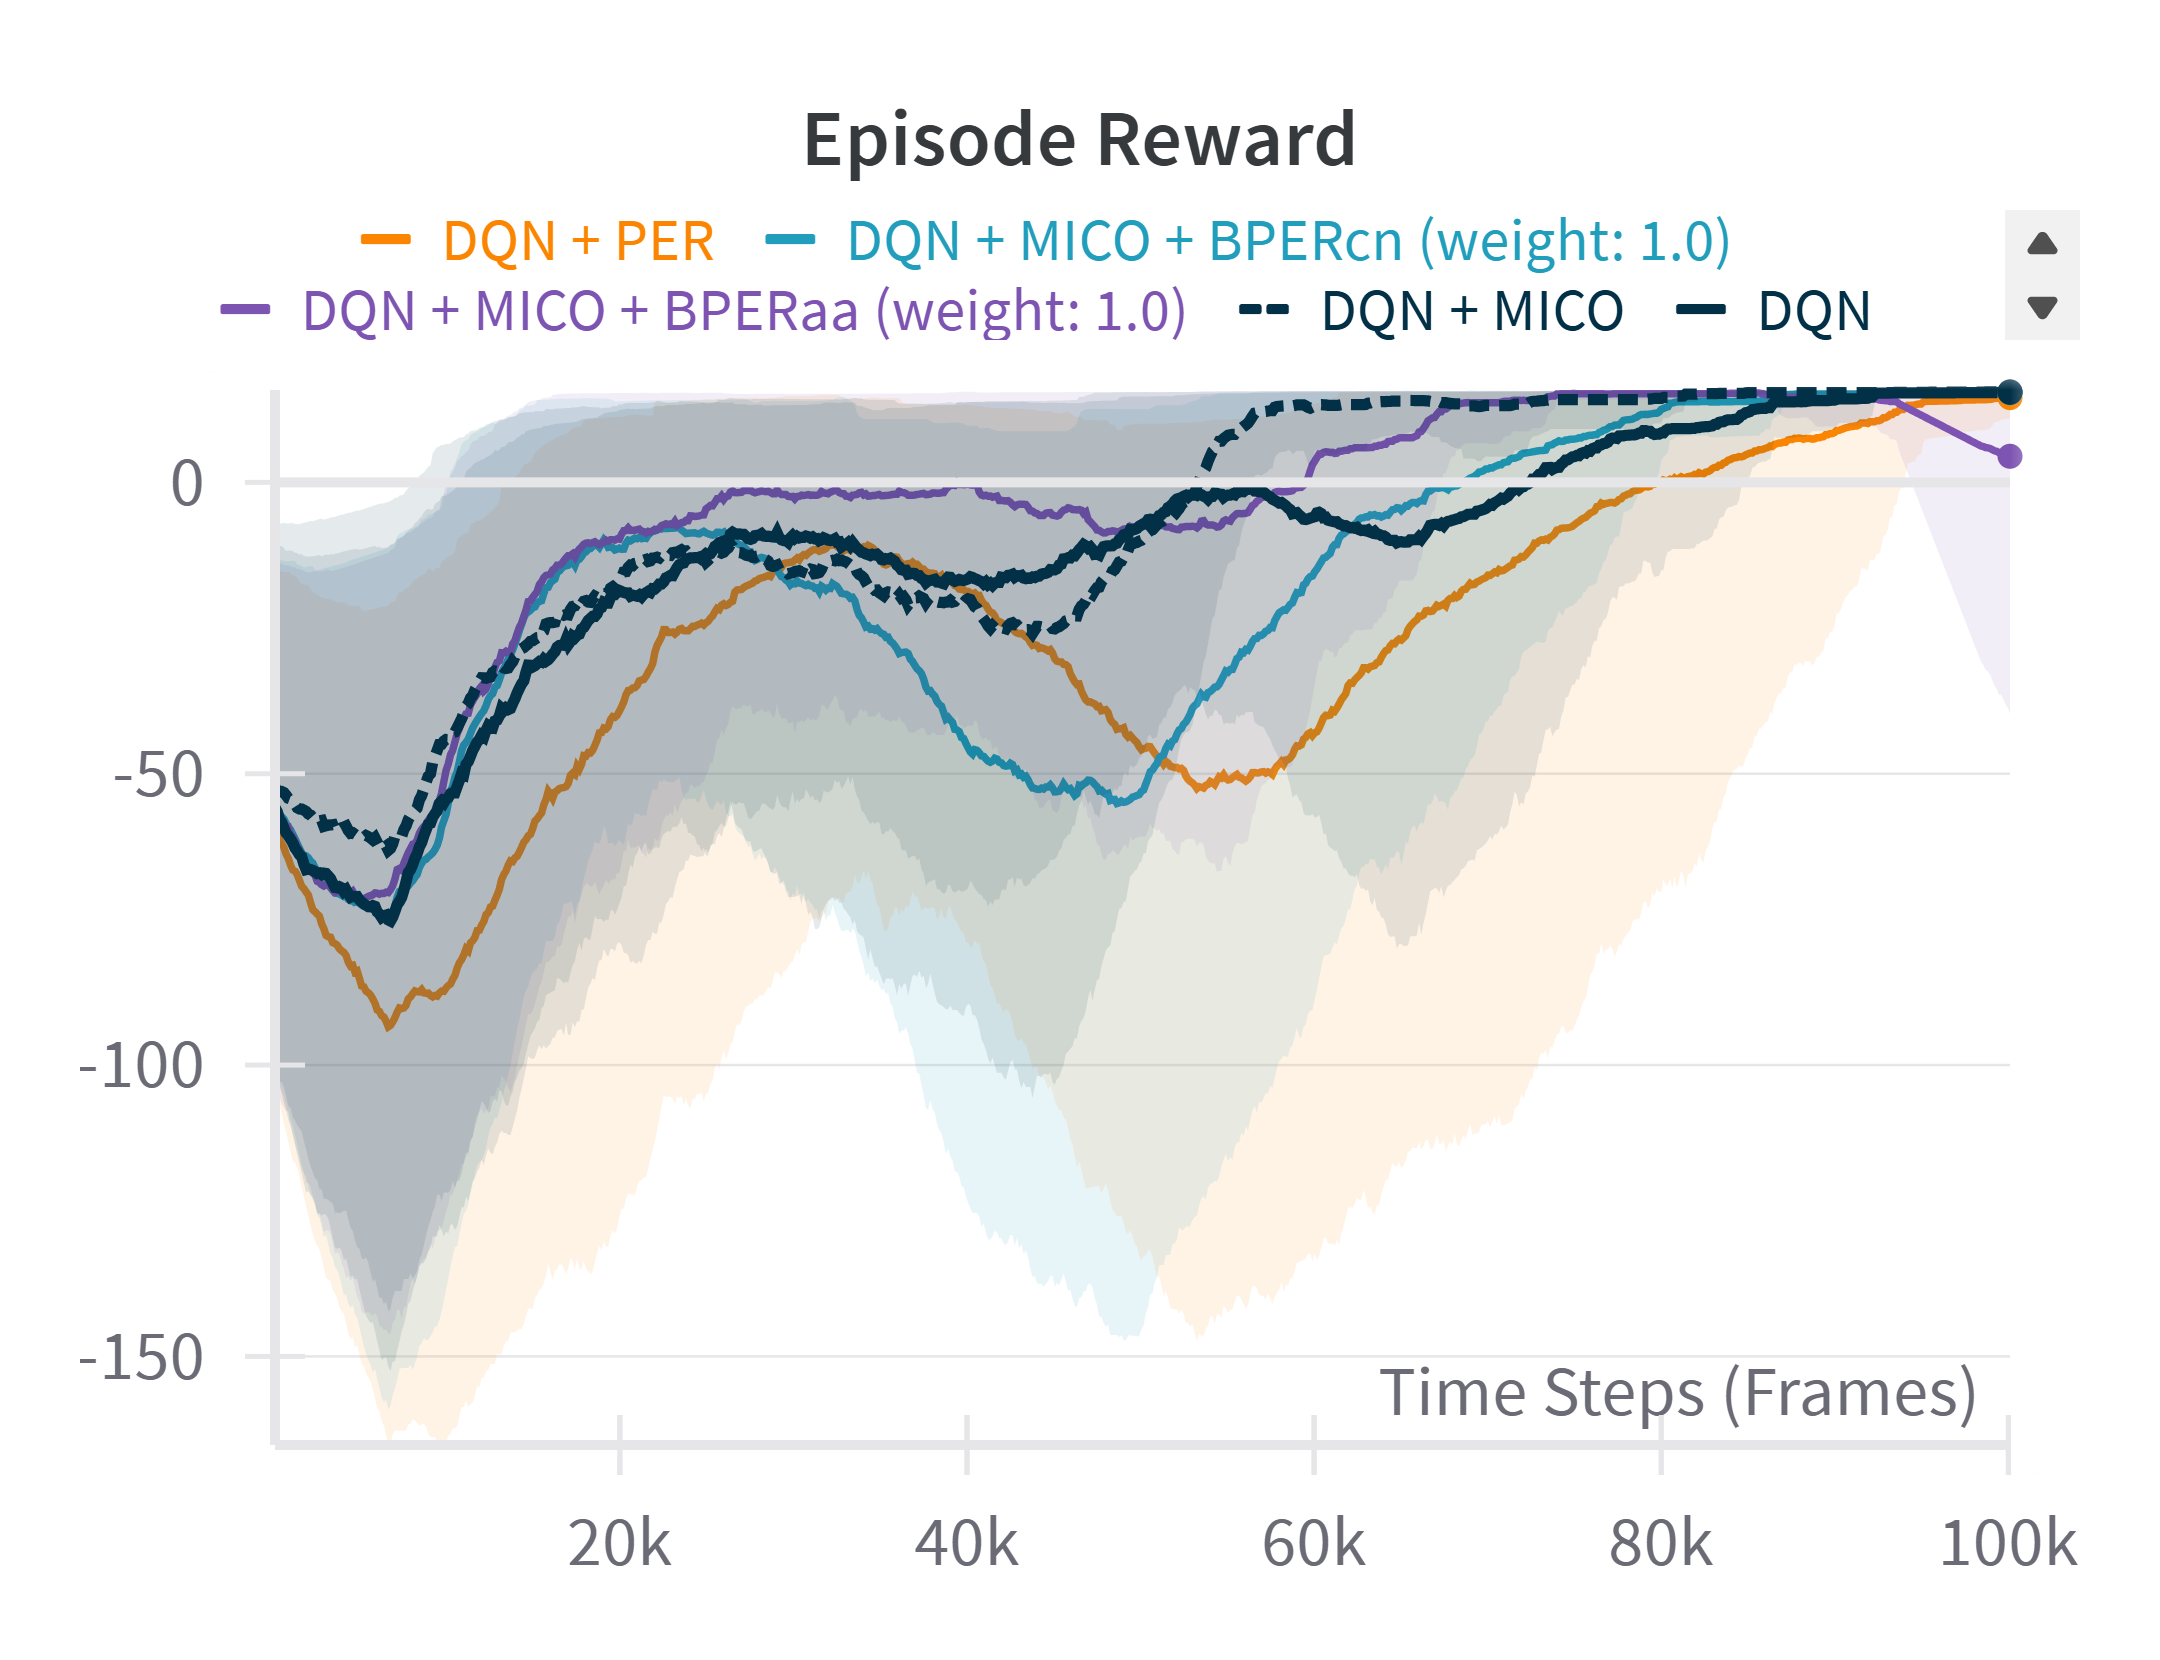
\includegraphics[width=\linewidth]{Results/grid_world/episode_reward_grid_world_window_100.png}
        \caption{Episode Reward}
        \label{fig:episode_reward_grid_world}
    \end{subfigure}
    \hfill
    \begin{subfigure}{0.45\textwidth}
        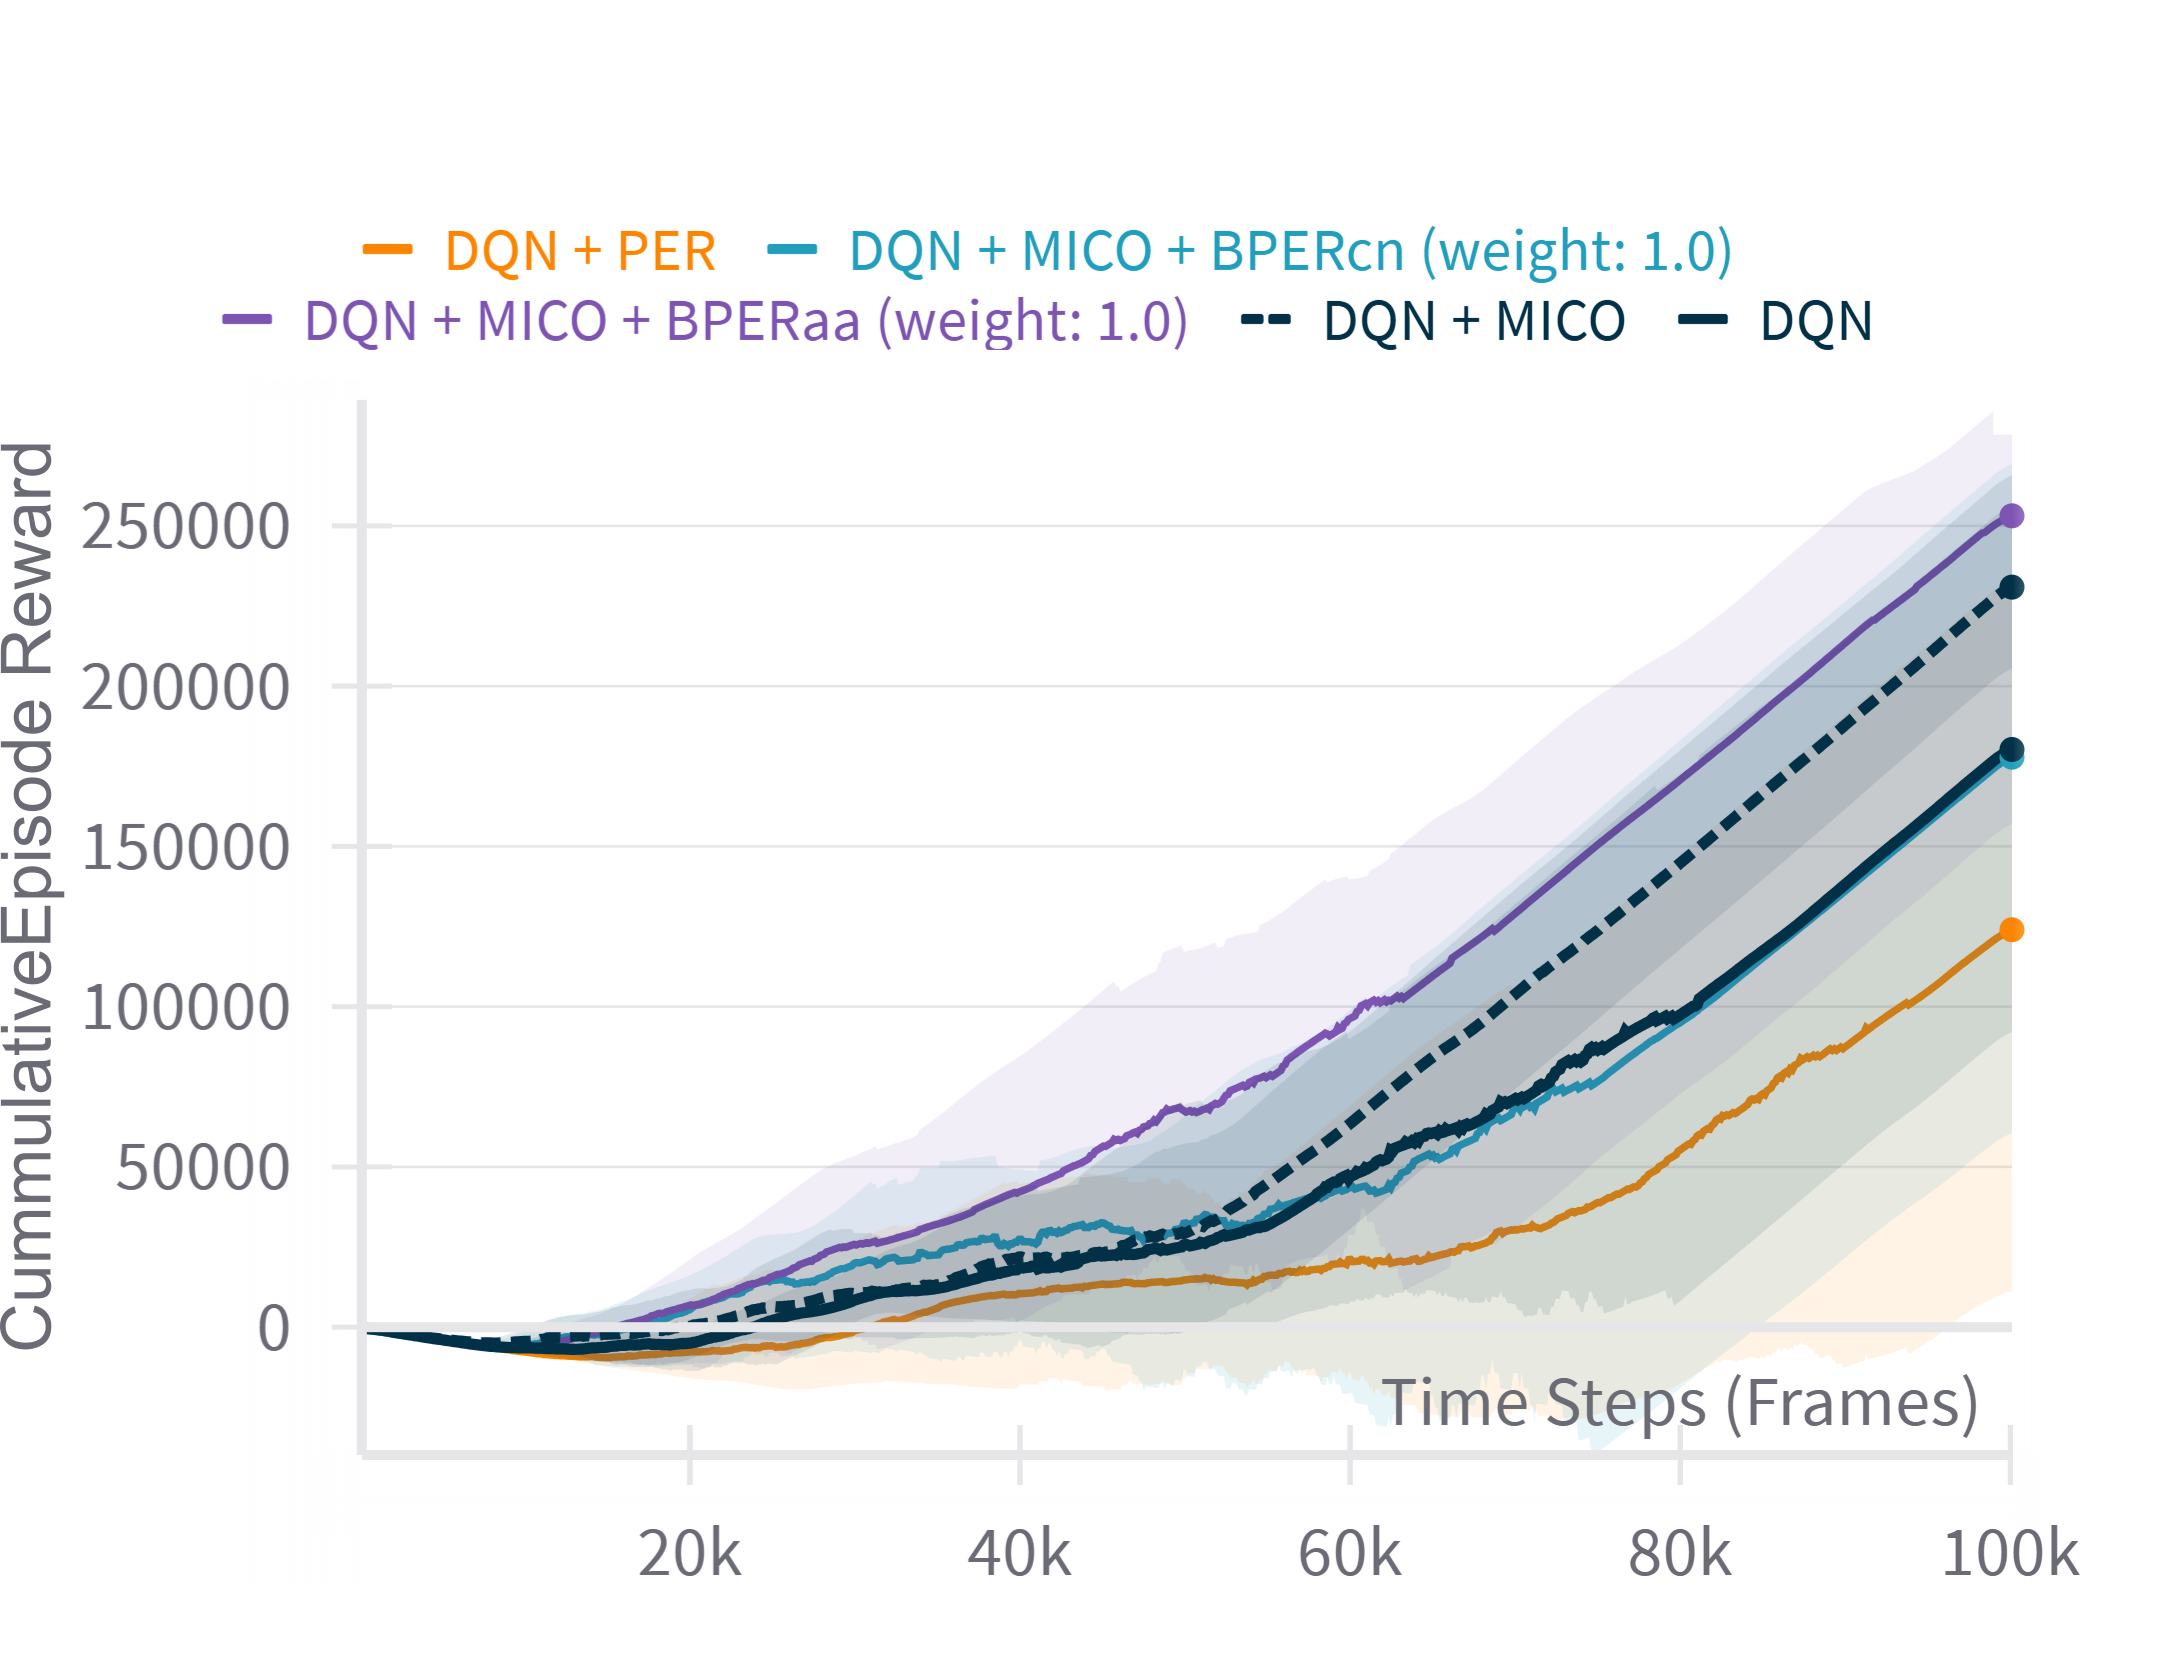
\includegraphics[width=\linewidth]{Results/grid_world/cumulative_episode_return.png}
        \caption{Cumulative Reward}
        \label{fig:cumulative_reward}
    \end{subfigure}
    \caption[Episode and Cumulative Reward]{\textbf{Episode and Cumulative Reward.} Reward performance comparison for different methods over time. The results represent the average from 5 independent executions, with shaded regions indicating the variability for each method.}
    \label{fig:cumulative_episode_reward}
\end{figure}

The cumulative reward, as shown in Figure \ref{fig:cumulative_reward}, indicates the total reward collected over time, which provides insight into the overall reward collection of each method. A higher cumulative reward indicates a better ability to select actions that lead to positive outcomes. The complementary results suggest that BPERaa produces a policy that consistently collects higher rewards, outperforming the direct baseline DQN + MICo, and demonstrating that BPERaa positively impacts DQN + MICo's performance. In contrast, the BPERcn strategy shows improvements in the early stages of learning but starts to decline around the 50k time step, reducing reward acquisition compared to DQN + MICo and eventually performing similarly to the baseline DQN. Overall, the PER method performs the worst, struggling to collect rewards and hindering the learning of the baseline DQN.

\begin{figure}[!h]
    \centering
    \begin{subfigure}{0.45\textwidth}
    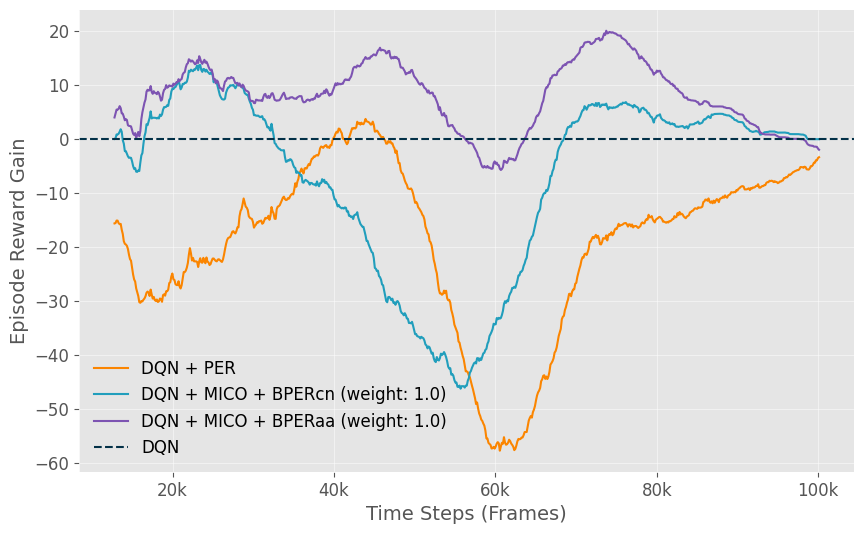
\includegraphics[width=\linewidth]{Results/grid_world/episode_reward_gain_baseline_dqn.png}
        \caption{Baseline DQN}
        \label{fig:episode_reward_gain_dqn}
    \end{subfigure}
    \hfill
    \begin{subfigure}{0.45\textwidth}
        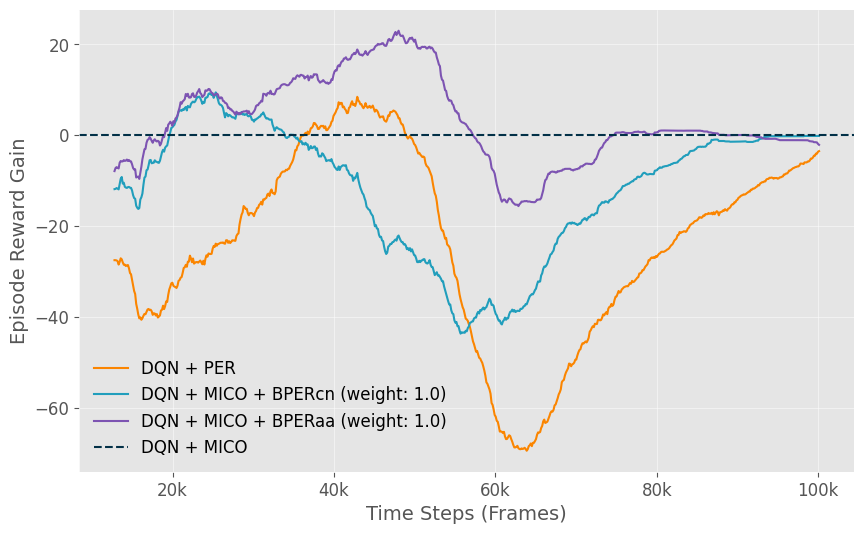
\includegraphics[width=\linewidth]{Results/grid_world/episode_reward_gain_baseline_dqn_mico.png}
        \caption{Baseline DQN + MICO}
        \label{fig:episode_reward_gain_dqn_mico}
    \end{subfigure}
    \caption{Episode Reward Gain }
    \label{fig:episode_reward_gain_dqn_and_mico}
\end{figure}

The episode reward gain, shown in Figure \ref{fig:episode_reward_gain_dqn_and_mico}, provides an alternative perspective for evaluating the improvement of the proposed methods relative to two baselines (DQN and DQN + MICo). Since the episode reward gain is the difference between the episode reward of a method and a baseline, a positive value indicates a better performance relative to the baseline. This evaluation metric is calculated using a moving average window of 100 episodes based on the mean episode reward previously shown in Figure \ref{fig:episode_reward_grid_world}. The results confirm the promising improvements of the BPERaa strategy over the other methods relative to both baselines. Both strategies, BPERaa and BPERcn, exhibit similar improvements in the early stages of training. However, the performance of BPERcn declines around the 30k step under both baselines. Interestingly, Figure \ref{fig:episode_reward_gain_dqn_mico} reveals a decreasing trend around the 50k step for the BPERaa method. Although the performance eventually recovers to match that of DQN + MICo, the decline suggests some instability. Under both baselines, the PER method significantly underperforms, hindering the effective learning of the policy.



\section{Task-agnostic Sampling}

This section aims to empirically demonstrate that the proposed method efficiently prioritizes samples based on their behavioral relevance. To achieve this, the on-policy bisimulation recurrent operator $T_K^\pi$ for deterministic environments (see Equation \ref{eq:deterministic_on_policy_bisimulation_metric}) is employed to compute exact on-policy bisimulation distances, providing a quantitative evaluation. In the experience replay, each transition is associated with the exact on-policy bisimulation distance between the current and next state. This exact distance effectively serves as a behavioral value indicator per transition, and allow us to assess the degree of behavioral similar or dissimilar transitions in an experience replay by plotting their distributions over time. The reader must keep in mind that these exact distances differ from the approximated distances used in the BPERcn strategy; while the BPERcn provides approximate measures, the operator $T_K^\pi$ offers 'theoretical' exact distances\footnote{Note that the calculation of the exact on-policy bisimulation distances is only feasible in this toy example, where the true states are fully known. In practice, such information is typically not accessible.}.

\begin{figure}[H]
    \centering
    \begin{subfigure}{0.32\textwidth}
    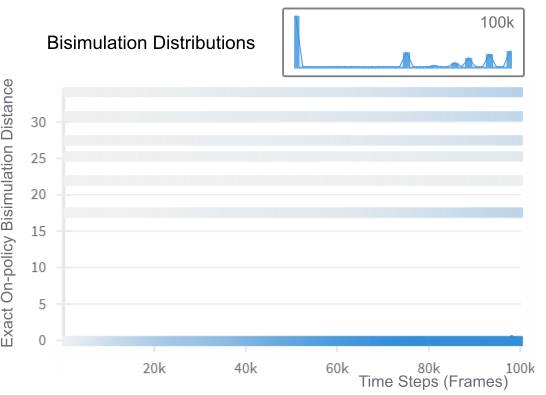
\includegraphics[width=\linewidth]{Results/grid_world/exact_bisimulation_dqn_per.png}
        \caption{DQN + PER}
        \label{fig:exact_bisim_per}
    \end{subfigure}
    \hfill
    \begin{subfigure}{0.32\textwidth}
        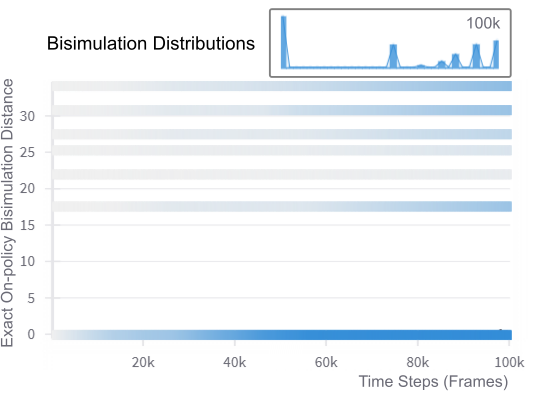
\includegraphics[width=\linewidth]{Results/grid_world/exact_bisimulation_dqn_mico_bpercn.png}
        \caption{DQN (MICO) + BPERcn}
        \label{fig:exact_bisim_bpercn}
    \end{subfigure}
    \hfill
    \begin{subfigure}{0.32\textwidth}
        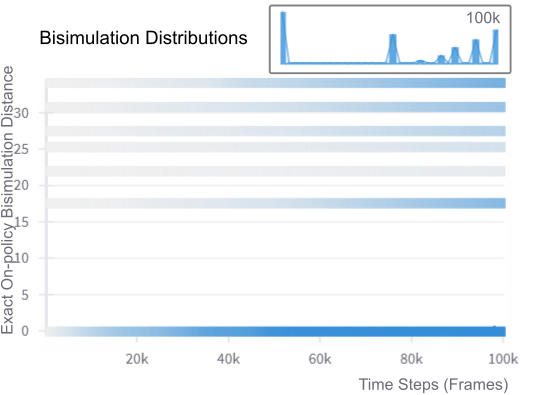
\includegraphics[width=\linewidth]{Results/grid_world/exact_bisimulation_dqn_mico_bperaa.png}
        \caption{DQN (MICO) + BPERaa}
        \label{fig:exact_bisim_bperaa}
    \end{subfigure}
    \caption{Two images side-by-side}
    \label{fig:exact_bisimulation_distributions}
\end{figure}


Figure \ref{fig:exact_bisimulation_distributions} illustrates the distribution of exact current-next on-policy bisimulation distances in the experience replay over time, with the final distribution (at 100k step) highlighted at the top of the figure. In both BPERcn and BPERaa strategies, the behavioral dissimilar transitions evolve to larger values compared to PER over time, specifically with exact bisimulation distance higher than 30 and between 15 and 20 more frequent in the experience replay. It clearly demonstrates how our method prioritizes more frequently those larger behavioral dissimilar transitions. As the BPERcn encourages highly dissimilar transition between the current and next states approximated during training, the results from Figure \ref{fig:exact_bisim_bpercn} are expected. However, a more interesting result is that despite of BPERaa prioritizes transitions based on relative priorities within the current mini-batch, this second strategy is still able to prioritize dissimilar experiences as efficiently as the strategy BPERcn (see Figure \ref{fig:exact_bisim_bperaa}).

Another interesting result is that, despite the methods aiming to prioritize highly dissimilar transitions, Figure \ref{fig:exact_bisimulation_distributions} still shows a significant number of transitions with exact bisimulation distances close to zero. This outcome could be attributed to the nature of the environment, which contains many highly similar states. Additionally, this result may be influenced by the use of a large buffer size of 100 000, which was deliberately set to a high capacity to observe behavior under large-scale conditions; more common in state-of-the-art methods.

Having established the distribution of behaviorally dissimilar transitions in the experience replay, the next step is to analyze how many of these transitions actually correspond to high priority values. To explore this, Figure \ref{fig:priority_distributions} illustrates the evolution of priority distributions in the experience replay over time, with the final distribution (at 100k steps) highlighted at the top.

\begin{figure}[H]
    \centering
    \begin{subfigure}{0.32\textwidth}
    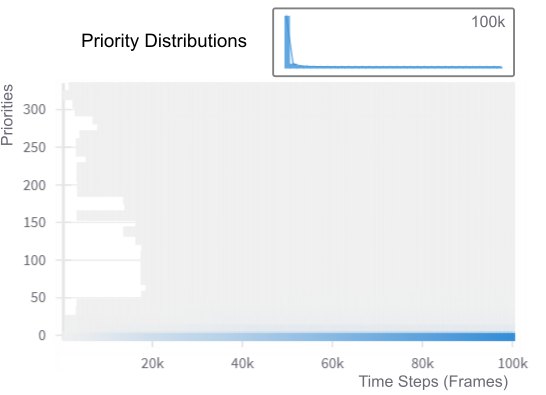
\includegraphics[width=\linewidth]{Results/grid_world/priority_distribution_dqn_per.png}
        \caption{DQN + PER}
        \label{fig:priority_distribution_per}
    \end{subfigure}
    \hfill
    \begin{subfigure}{0.32\textwidth}
        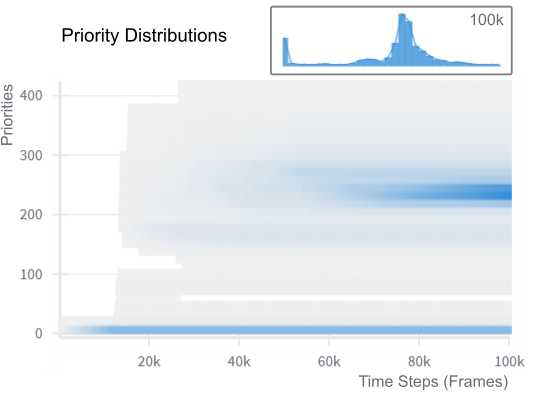
\includegraphics[width=\linewidth]{Results/grid_world/priority_distribution_dqn_mico_bpercn.png}
        \caption{DQN (MICO) + BPERcn}
        \label{fig:priority_distribution_bpercn}
    \end{subfigure}
    \hfill
    \begin{subfigure}{0.32\textwidth}
        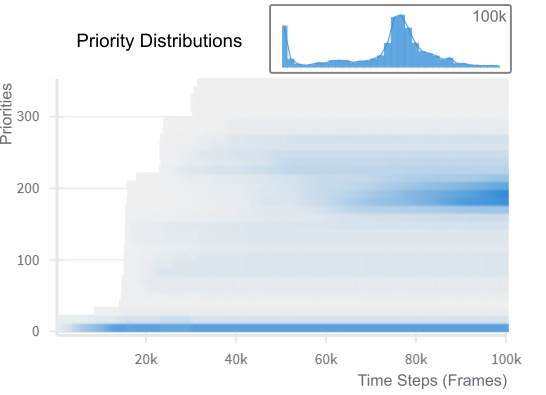
\includegraphics[width=\linewidth]{Results/grid_world/priority_distribution_dqn_mico_bperaa.png}
        \caption{DQN (MICO) + BPERaa}
        \label{fig:priority_distribution_bperaa}
    \end{subfigure}
    \caption{Two images side-by-side}
    \label{fig:priority_distributions}
\end{figure}

Figure \ref{fig:priority_distribution_per} shows an accumulation of low priority values over time in the PER method, with relatively few higher priority values. Although those priority values are low close to zero, their combined effect can occupy a large portion of the probability area, resulting in transitions with low TD-error being sampled more frequently. This phenomenon hinders DQN learning and may explain the poor episode rewards observed in previous experiments. In contrast, both proposed strategies, BPERcn and BPERaa, consistently generate higher priority values over time, encouraging more behaviorally dissimilar transitions, compensating the accumulation of low priority values. Notably, BPERaa exhibits slightly greater variability in Figure \ref{fig:priority_distribution_bperaa}. Despite of BPERcn and BPERaa still exhibiting an accumulation of low priority values, their frequency is lower compared to the PER method. While these results do not directly associate each priority value with the exact bisimulation distances mentioned earlier, they provide insight into how many behaviorally dissimilar transitions in the experience replay are being prioritized over time.

\begin{figure}[p]
    \centering
    \begin{subfigure}{1.\textwidth}
    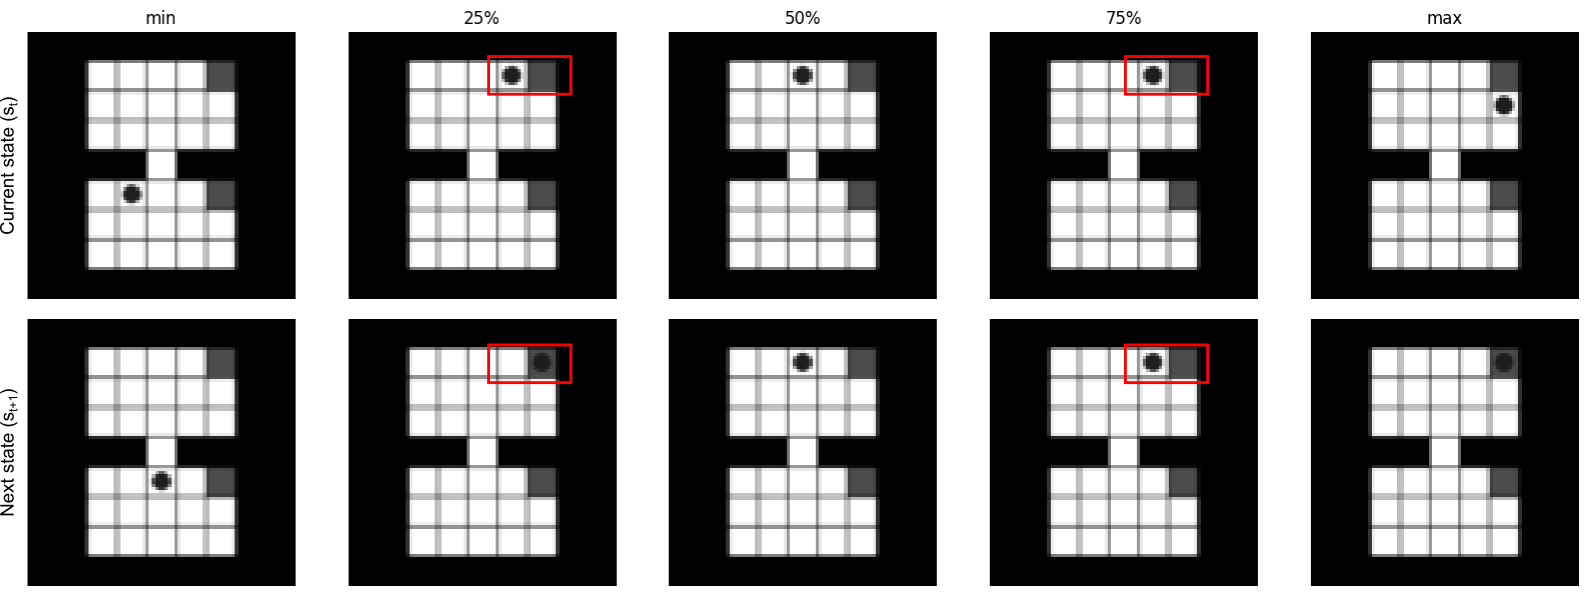
\includegraphics[width=\linewidth]{Results/grid_world/quartiles_images_per.png}
        \caption{DQN + PER}
        \label{fig:quartiles_per}
    \end{subfigure}
    \begin{subfigure}{1.\textwidth}
        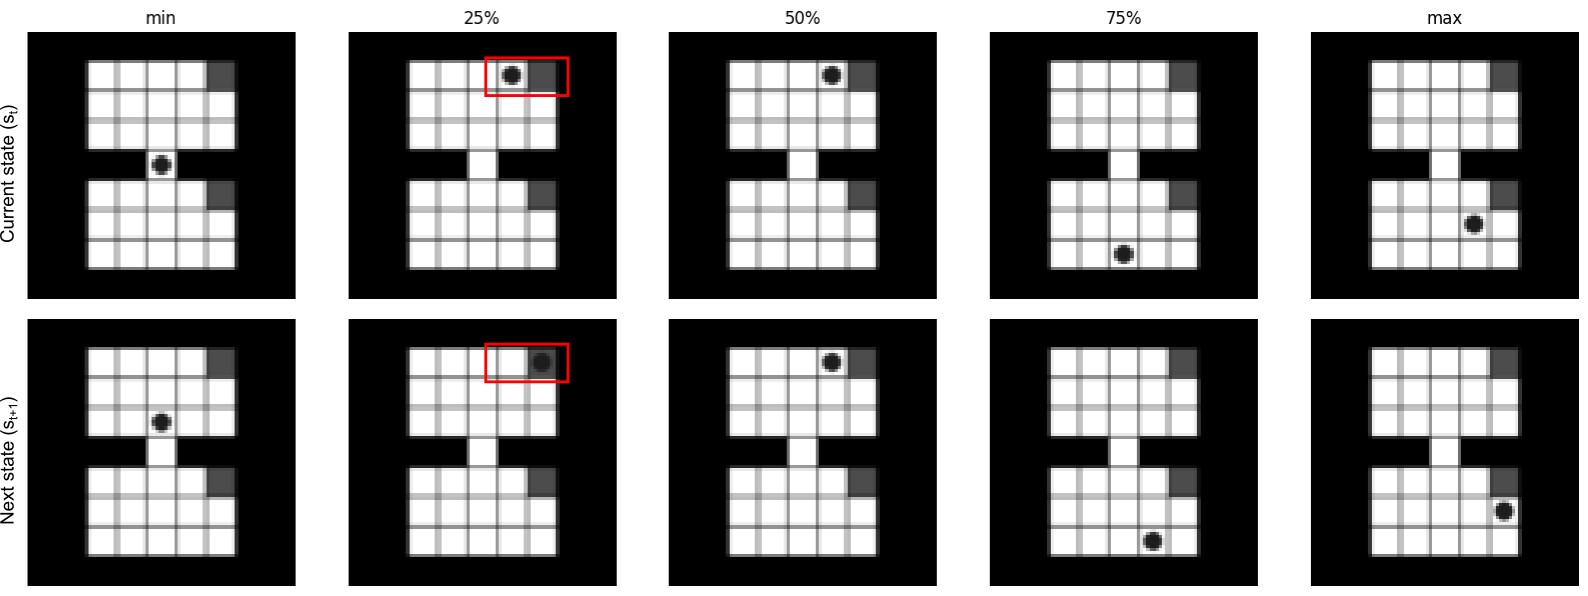
\includegraphics[width=\linewidth]{Results/grid_world/quartiles_images_dqn_mico_bpercn.png}
        \caption{DQN (MICO) + BPERcn}
        \label{fig:quartiles_bpercn}
    \end{subfigure}
    \begin{subfigure}{1.\textwidth}
        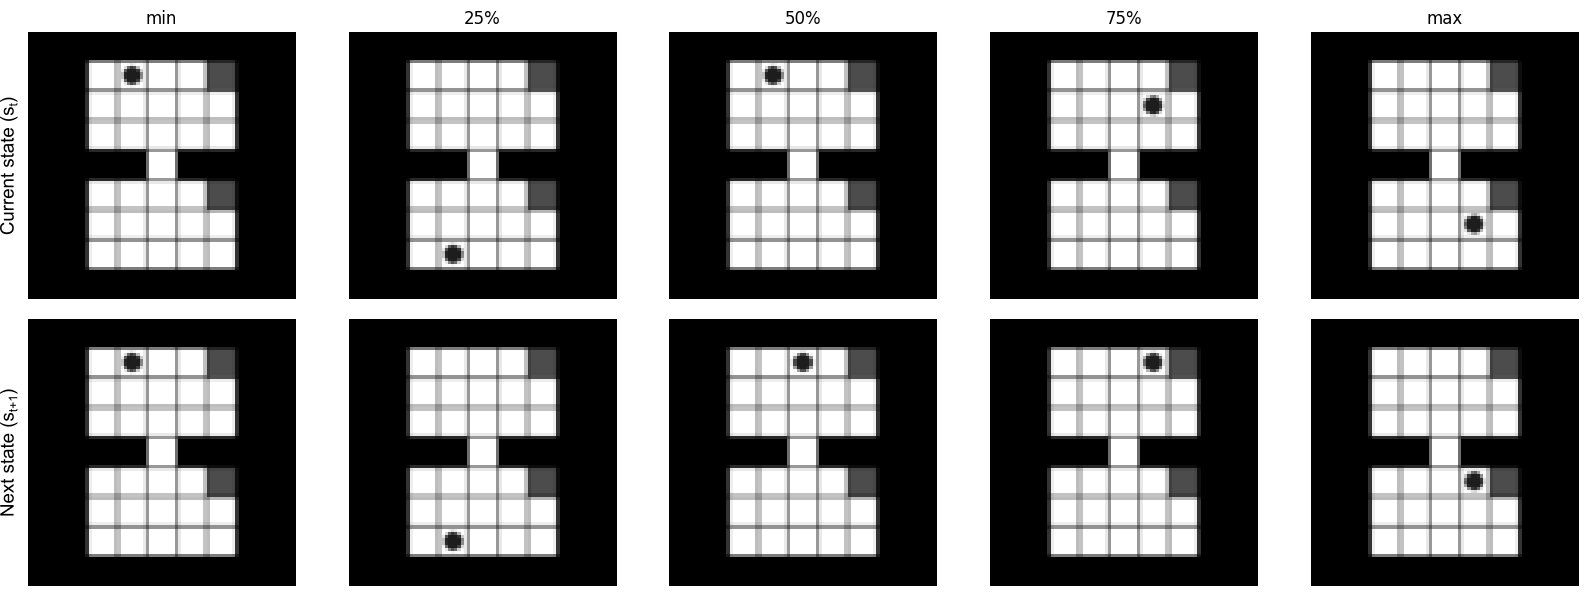
\includegraphics[width=\linewidth]{Results/grid_world/quartiles_images_dqn_mico_bperaa.png}
        \caption{DQN (MICO) + BPERaa}
        \label{fig:quartiles_bperaa}
    \end{subfigure}
    \caption{Two images side-by-side}
    \label{fig:quartiles_all_methods}
\end{figure}

\subsection{Visual Inspection}

% Later, Figure \ref{fig:quartiles_all_methods} show a qualitative visual inspection of the frames corresponding to the main quartiles priorities values in the experience replay in the time step 90k. The low quartiles (min, 25\%) corresponds to frames with low sampling probability, and higher quartiles (75\% and max) corresponds to frames with higher sampling probability. The top row corresponds to the current states and the bottom row corresponds to the next states in each transition. 

% Figure \ref{algorithm:dqn_per} exhibits the aforementioned difficulties of PER method when trying to prioritized state transitions using the td-error. In the quartile 25\% transition, the algorithm assigns low value priority to a transition that reach the goal, while assign high priority in the quartile 75\% to a transition that gets stuck in the same position without reaching the goal; clearly leading to a low expected learning progress. On the contrary, the strategies BPERcn and BPERaa show a consistencies along the low quartiles by keeping lower priorities to transition that get stuck or going backwards with the goal, while keeping higher priorities to transition that moves towards the goal in the high quartiles. Notice, however, it seems to be small variances, specially in BPERcn where in the quartile 25\% we can see a lower transition probability assigned to a transition that leads towards the goal; suggesting scarce high priorities problems. For reference an additional visual inspection of the quartiles in the time step 50k is show in the Appendix \ref{}. 


Figure \ref{fig:quartiles_all_methods} provides a qualitative visual inspection of the frames corresponding to the main quartiles of priority values in the experience replay collected at the 90k time step. The lower quartiles (min and 25\%) represent frames with low sampling probabilities, while the higher quartiles (75\% and max) represent frames with higher sampling probabilities. The top row shows the current states, and the bottom row shows the next states for each transition.

Figure \ref{fig:quartiles_per} illustrates the difficulties of the PER method when attempting to prioritize state transitions using the TD-error. In the 25\% quartile transition, the algorithm assigns a low priority to a transition that reaches the goal, while assigning a high priority in the 75\% quartile to a transition where the agent is stuck in the same position without reaching the goal, clearly resulting in low expected learning progress. In contrast, the BPERcn and BPERaa strategies, show in Figures \ref{fig:quartiles_bpercn}, \ref{fig:quartiles_bperaa}, demonstrate consistency in the lower quartiles by assigning lower priorities to transitions where the agent gets stuck or moves backward relative to the goal, while maintaining higher priorities for transitions that move towards the goal in the higher quartiles. However, the BPERcn method shows small variances in the 25\% quartile, where a lower priority is assigned to a transition that leads towards the goal, suggesting occasional \textbf{issues with assigning high priorities}. For reference, an additional visual inspection of the quartiles at the 50k time step is provided in Appendix \ref{}.



% Notice that we could allegate that the low prioritization of the two quartiles makes sense because they could be associated with a small td-error; however, this is not necessarily true. In fact, accorsing previous Figure \ref{fig:episode_reward_grid_world}, there is still room for learning in the time step 90k for the DQN + PER algorithm.


\section{Outdated Priorities}

This section aims to empirically demonstrate that the proposed method alleviates the problem of outdated priorities. Recall that outdated priorities occur because priority updates are performed only on the current minibatch, rather than across the entire experience replay or, ideally, the whole state space. As a result, not all priorities are updated, leading to differences in sampling probability distributions. In this experiment, we measure this difference by comparing the distance between the ideal priority distribution (where priorities are updated across the entire state space under the current policy) and the approximated sampling priorities of the experience replay, as discussed in Section \ref{sec:experimental_setup}.

Figures \ref{fig:priority_dist_distance_on_policy_weighting} and \ref{fig:priority_dist_distance_uniform_weighting} show the on-policy and uniform weighting schemes respectively for calculating the distance between the ideal and approximated priority distributions,   averaged over 5 independent executions over time. The PER method exhibits greater distances over time than the BPERcn and BPERaa strategies, which also show less variability among executions. Although our method does not provides distances close to zero (such as Pan et al.'s work \cite{pan2022understanding}) indicating a perfect match between distributions, our method reduce and alleviate significantly the difference between the distributions without relying on model-based technique. 

\begin{figure}[!h]
    \centering
    \begin{subfigure}{0.45\textwidth}
    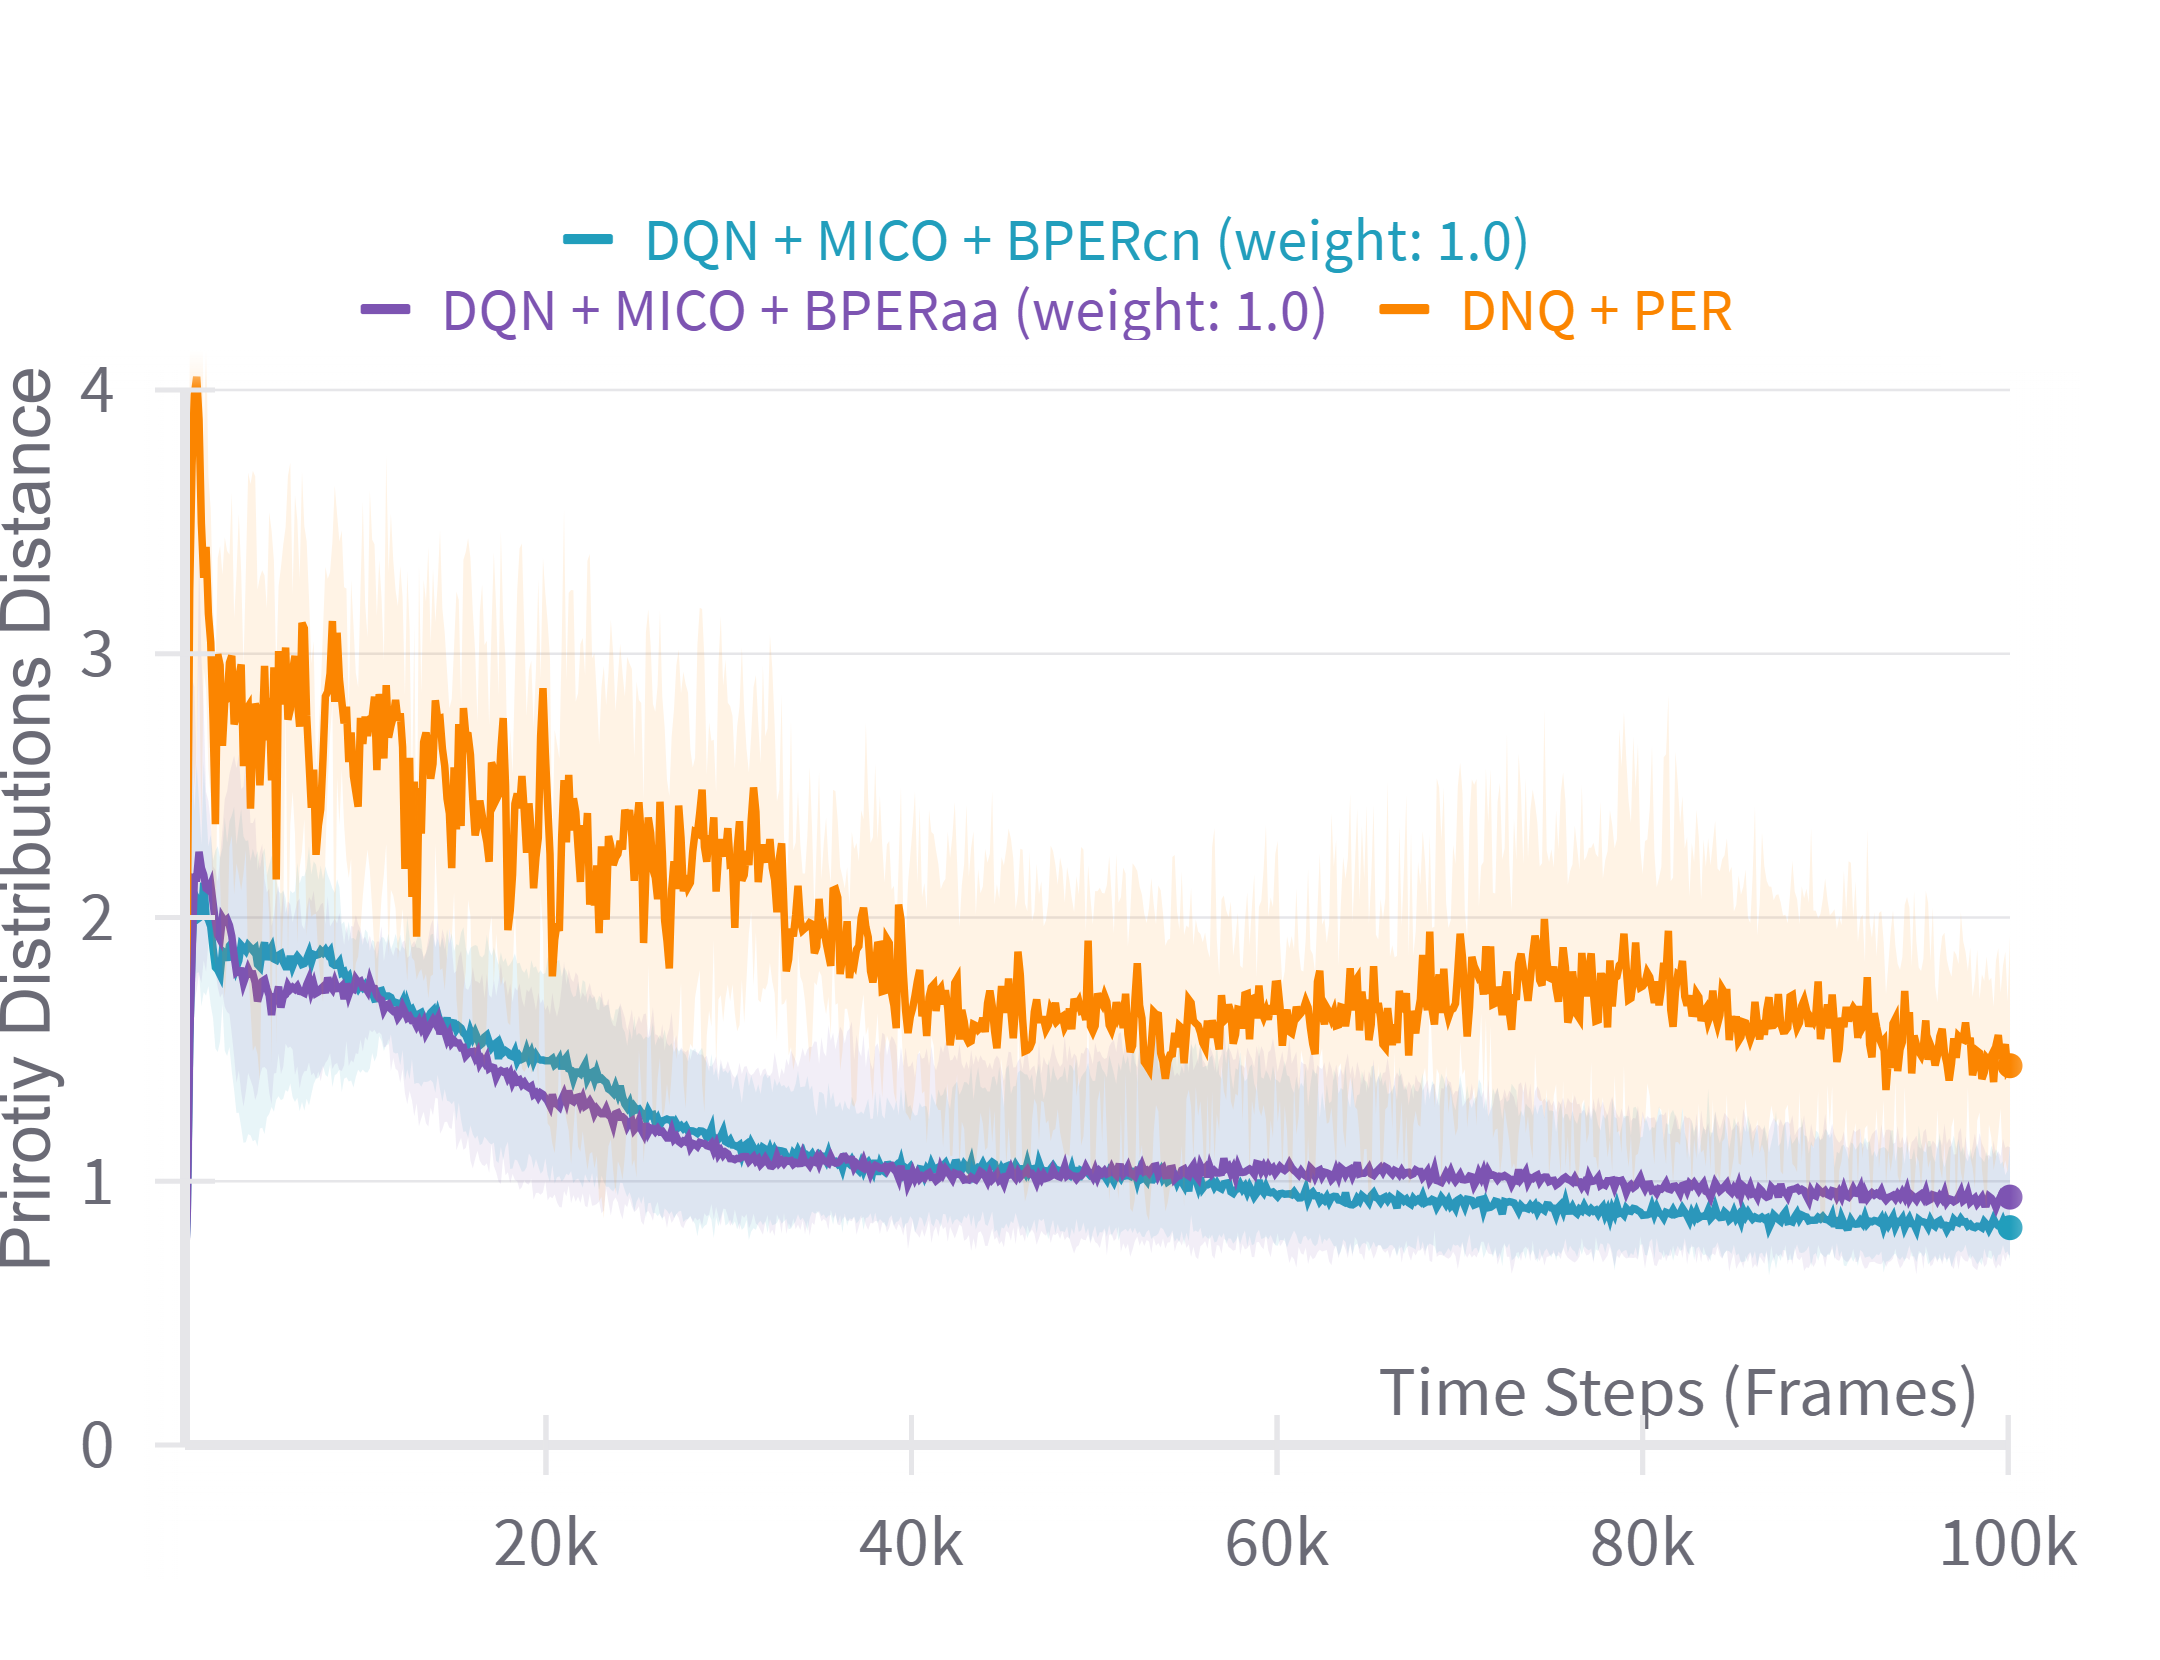
\includegraphics[width=\linewidth]{Results/grid_world/on_policy_weighting_outdated_priorities.png}
        \caption{On-policy Weighting}
        \label{fig:priority_dist_distance_on_policy_weighting}
    \end{subfigure}
    \hfill
    \begin{subfigure}{0.45\textwidth}
        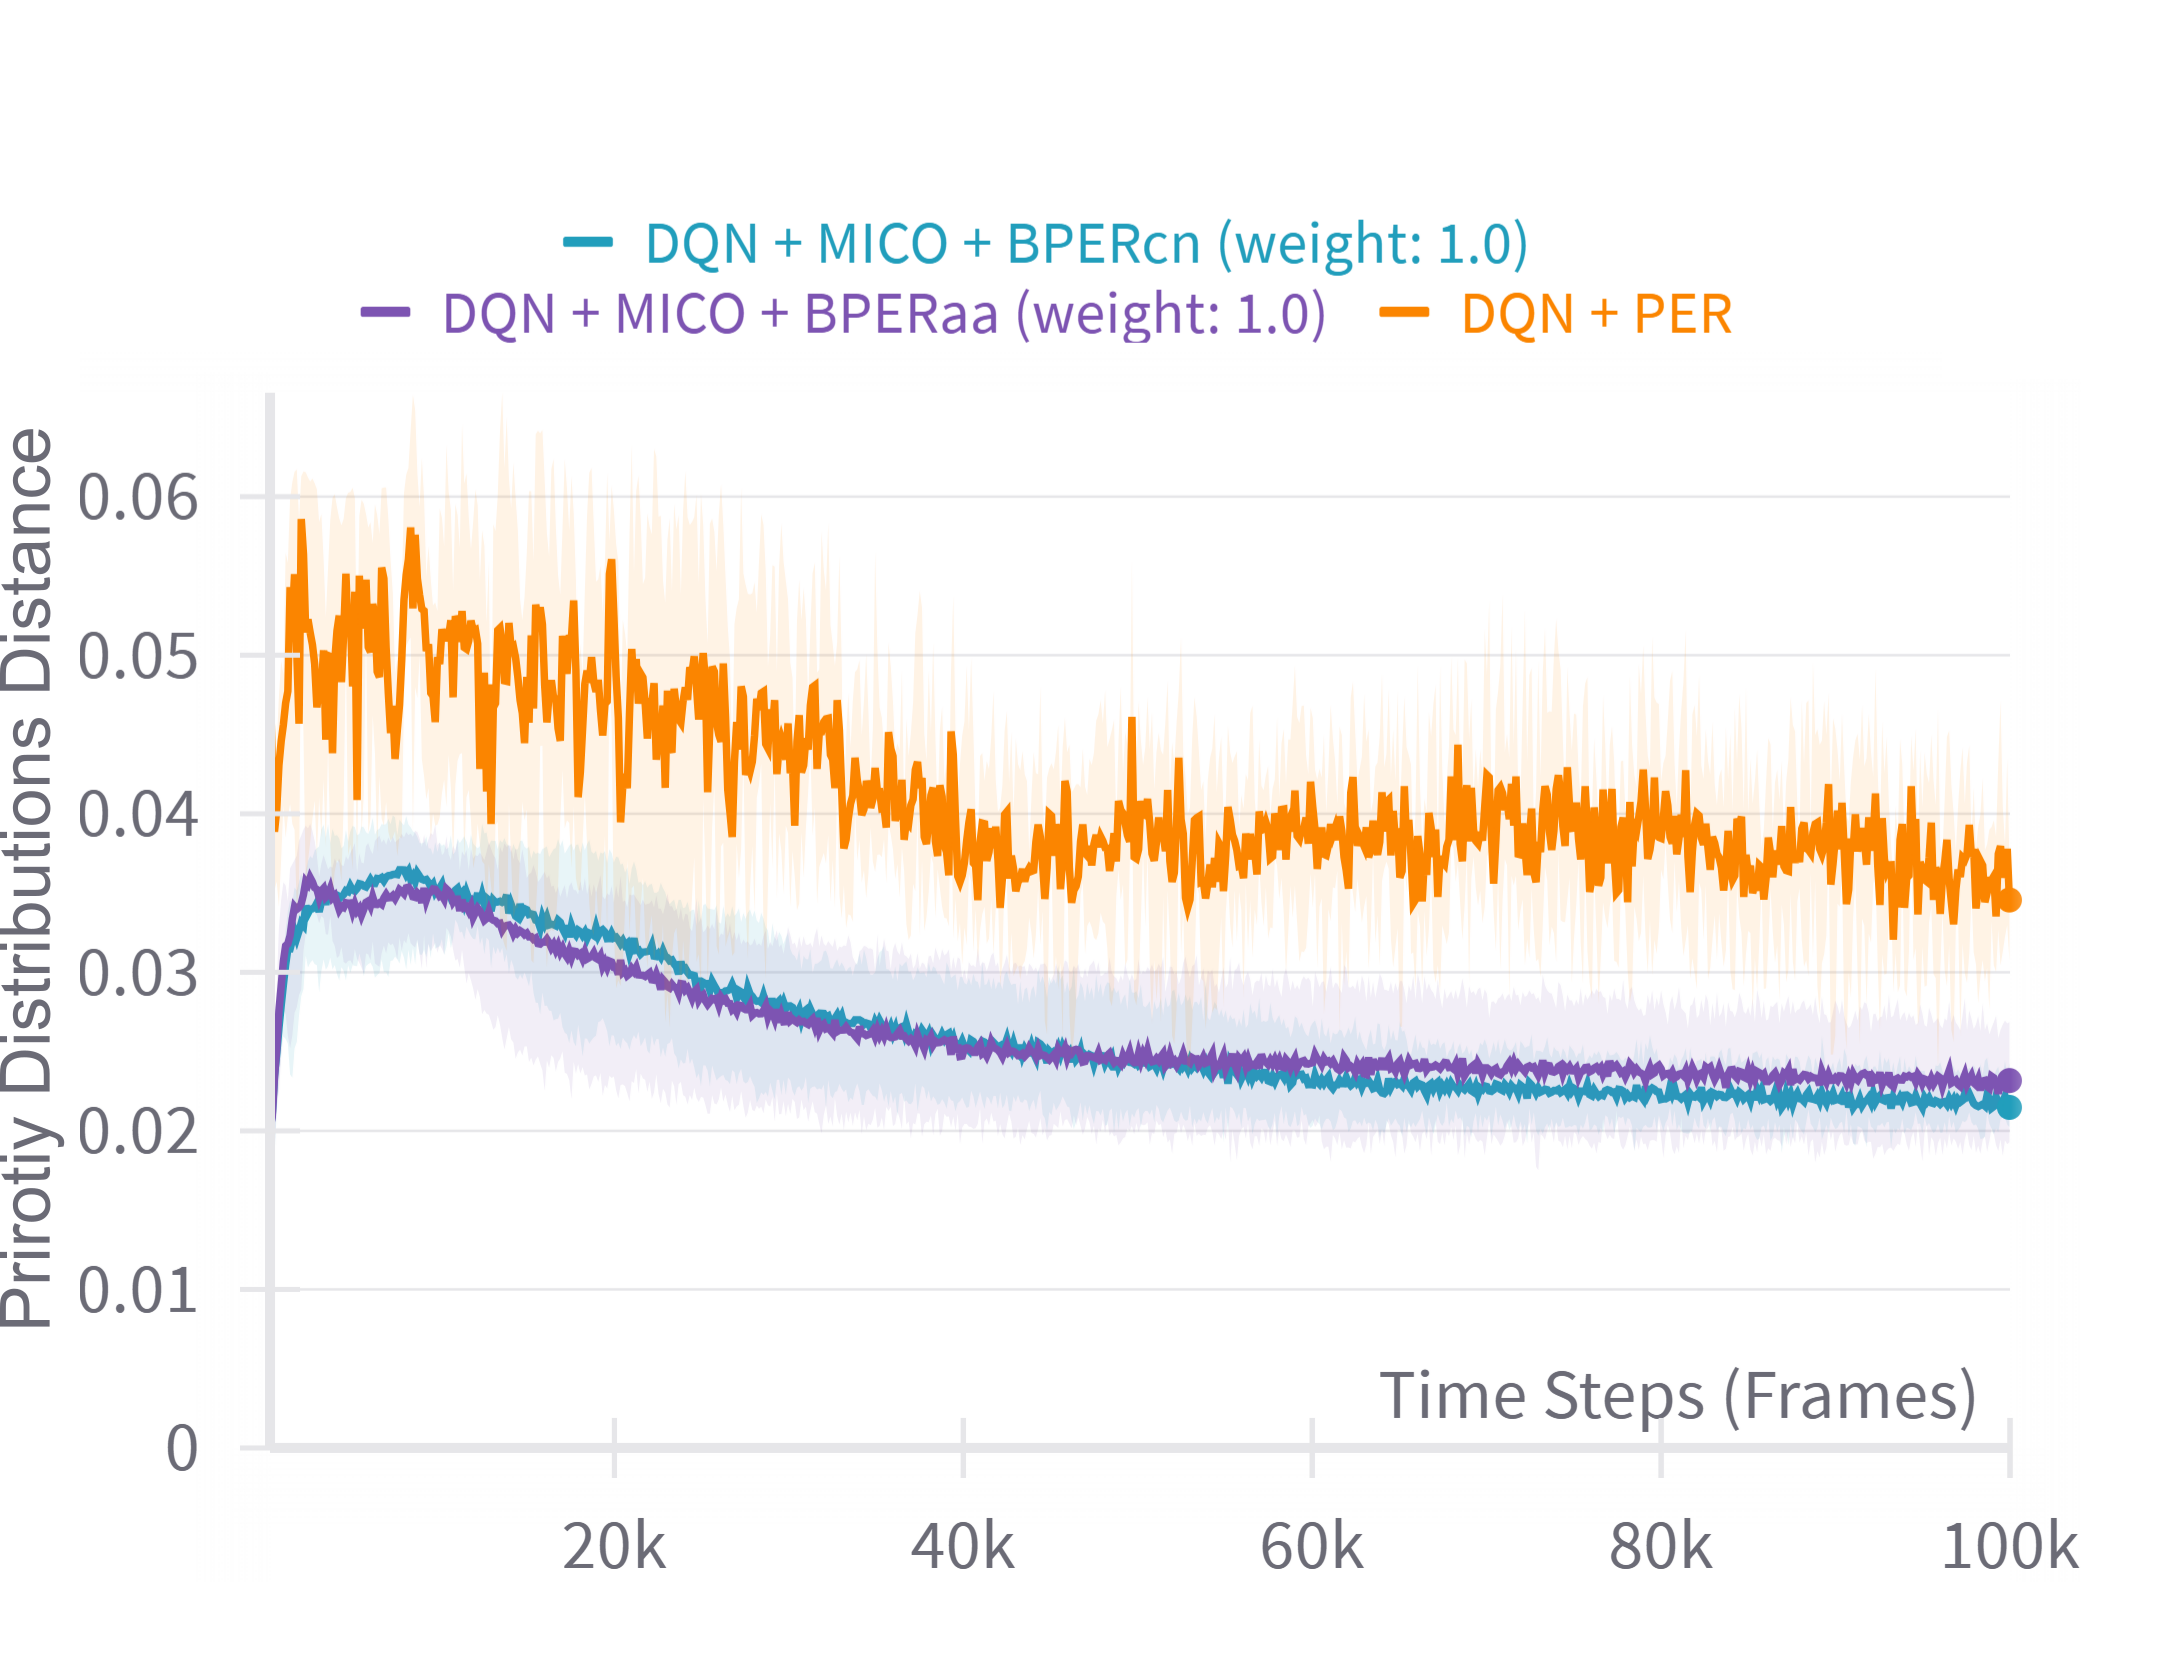
\includegraphics[width=\linewidth]{Results/grid_world/uniform_weighting_outdated_priorities.png}
        \caption{Uniform Weighting}
        \label{fig:priority_dist_distance_uniform_weighting}
    \end{subfigure}
    \caption{Two images side-by-side}
    \label{fig:priority_dist_distance}
\end{figure}

\section{State Space Coverage}

This section aims to empirically evaluate how our method addresses the state space coverage problem. The state space coverage problem arises from insufficient exploration, where the experience replay only captures a limited number of possible states, leading to suboptimal learning outcomes.

Figure \ref{fig:visitation_distributions} shows the state visitation distribution at the 90k time step in the 31-state Grid World, where cell values corresponds to the visit count per state. The results indicate that the strategies BPERcn and BPERaa visit more states more frequently compared to other methods, with BPERcn performing slightly better than BPERaa. Additionally, the DQN + MICO baseline outperforms DQN, and DQN + PER methods. While some of the increased exploration in BPERcn and BPERaa may be attributed to the MICo learning, the bisimulation prioritized technique further enhances exploration (relative to DQN + MICo) by significantly increasing the state visit counts, reaching values around 600.

% To evaluate a consistency among different runs, the Visitation Entropy mentioned in Section \ref{sec:experimental_setup} is used. 
Figure \ref{fig:visitation_entropy} illustrates the Visitation Entropy calculated from the visitations counts and average over 5 independent runs over time. A high entropy indicates that visitation distributions are more dispersed, consequently working as a indicator of exploration. While higher the entropy, better the exploration. The results clearly showcases that BPERaa outperforms the other methods with a large and consistent entropy, while the BPERcn although initially performs efficiently its performance decays around the time step 30k. PER method is the worse among all the methods. 


\begin{figure}[H]
    \centering
    % Add horizontal space to center the first two subfigures
    \hspace*{\fill}
    \begin{subfigure}{0.45\textwidth}
        \centering % Center the individual subfigure
        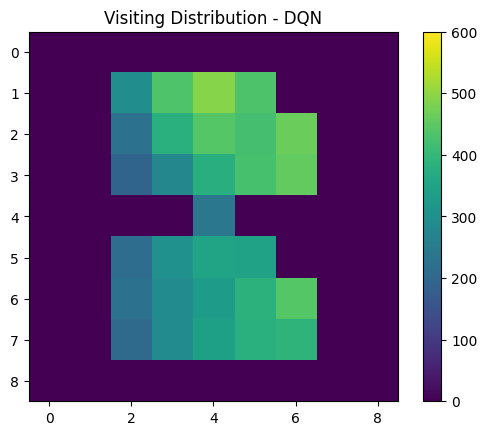
\includegraphics[width=0.70\linewidth]{Results/grid_world/visitation_distribution_dqn.png}
        \caption{DQN}
        \label{fig:visitation_distributions_dqn}
    \end{subfigure}
    \hspace*{\fill} % Adjust space between subfigures
    \begin{subfigure}{0.45\textwidth}
        \centering % Center the individual subfigure
        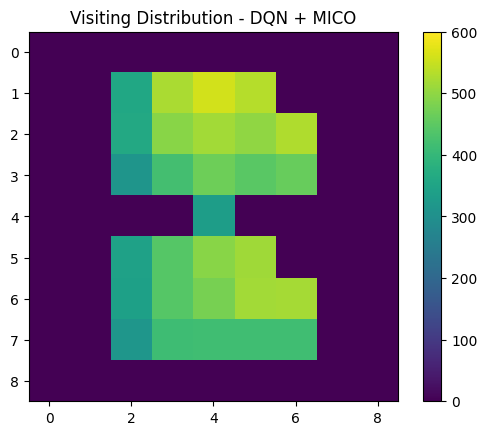
\includegraphics[width=0.70\linewidth]{Results/grid_world/visitation_distribution_dqn_mico.png}
        \caption{DQN + MICO}
        \label{fig:visitation_distributions_mico}
    \end{subfigure}
    \hspace*{\fill} % Add horizontal space to center the first two subfigures
    \vfill
    \begin{subfigure}{0.32\textwidth}
        \centering
        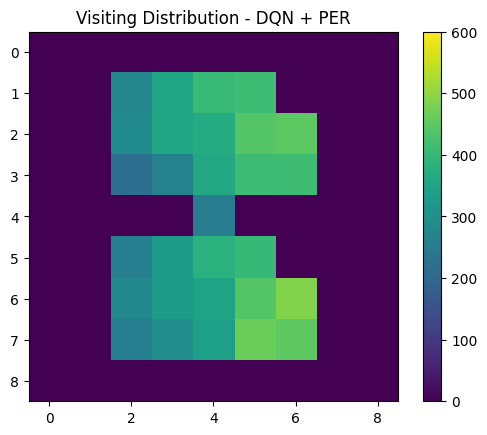
\includegraphics[width=\linewidth]{Results/grid_world/visitation_distribution_dqn_per.png}
        \caption{DQN + PER}
        \label{fig:visitation_distributions_per}
    \end{subfigure}
    \hfill
    \begin{subfigure}{0.32\textwidth}
        \centering
        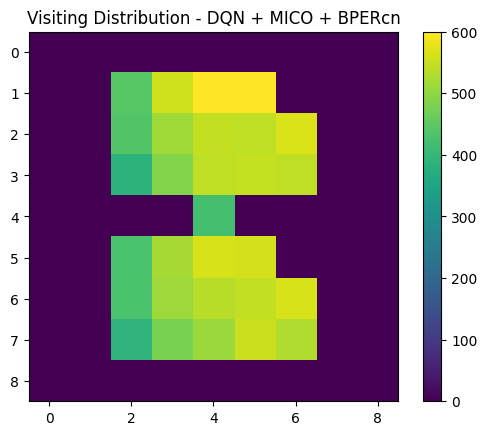
\includegraphics[width=\linewidth]{Results/grid_world/visitation_distribution_dqn_mico_bpercn.png}
        \caption{DQN + MICO + BPERcn}
        \label{fig:visitation_distributions_bpercn}
    \end{subfigure}
    \hfill
    \begin{subfigure}{0.32\textwidth}
        \centering
        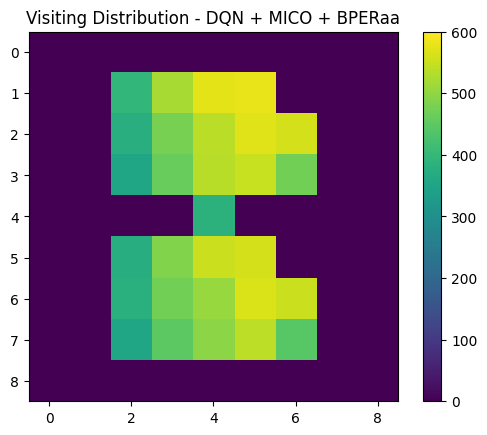
\includegraphics[width=\linewidth]{Results/grid_world/visitation_distribution_dqn_mico_bperaa.png}
        \caption{DQN + MICO + BPERaa}
        \label{fig:visitation_distributions_bperaa}
    \end{subfigure}
    \caption{Two images side-by-side}
    \label{fig:visitation_distributions}
\end{figure}

\begin{figure}[H]
    \centering
    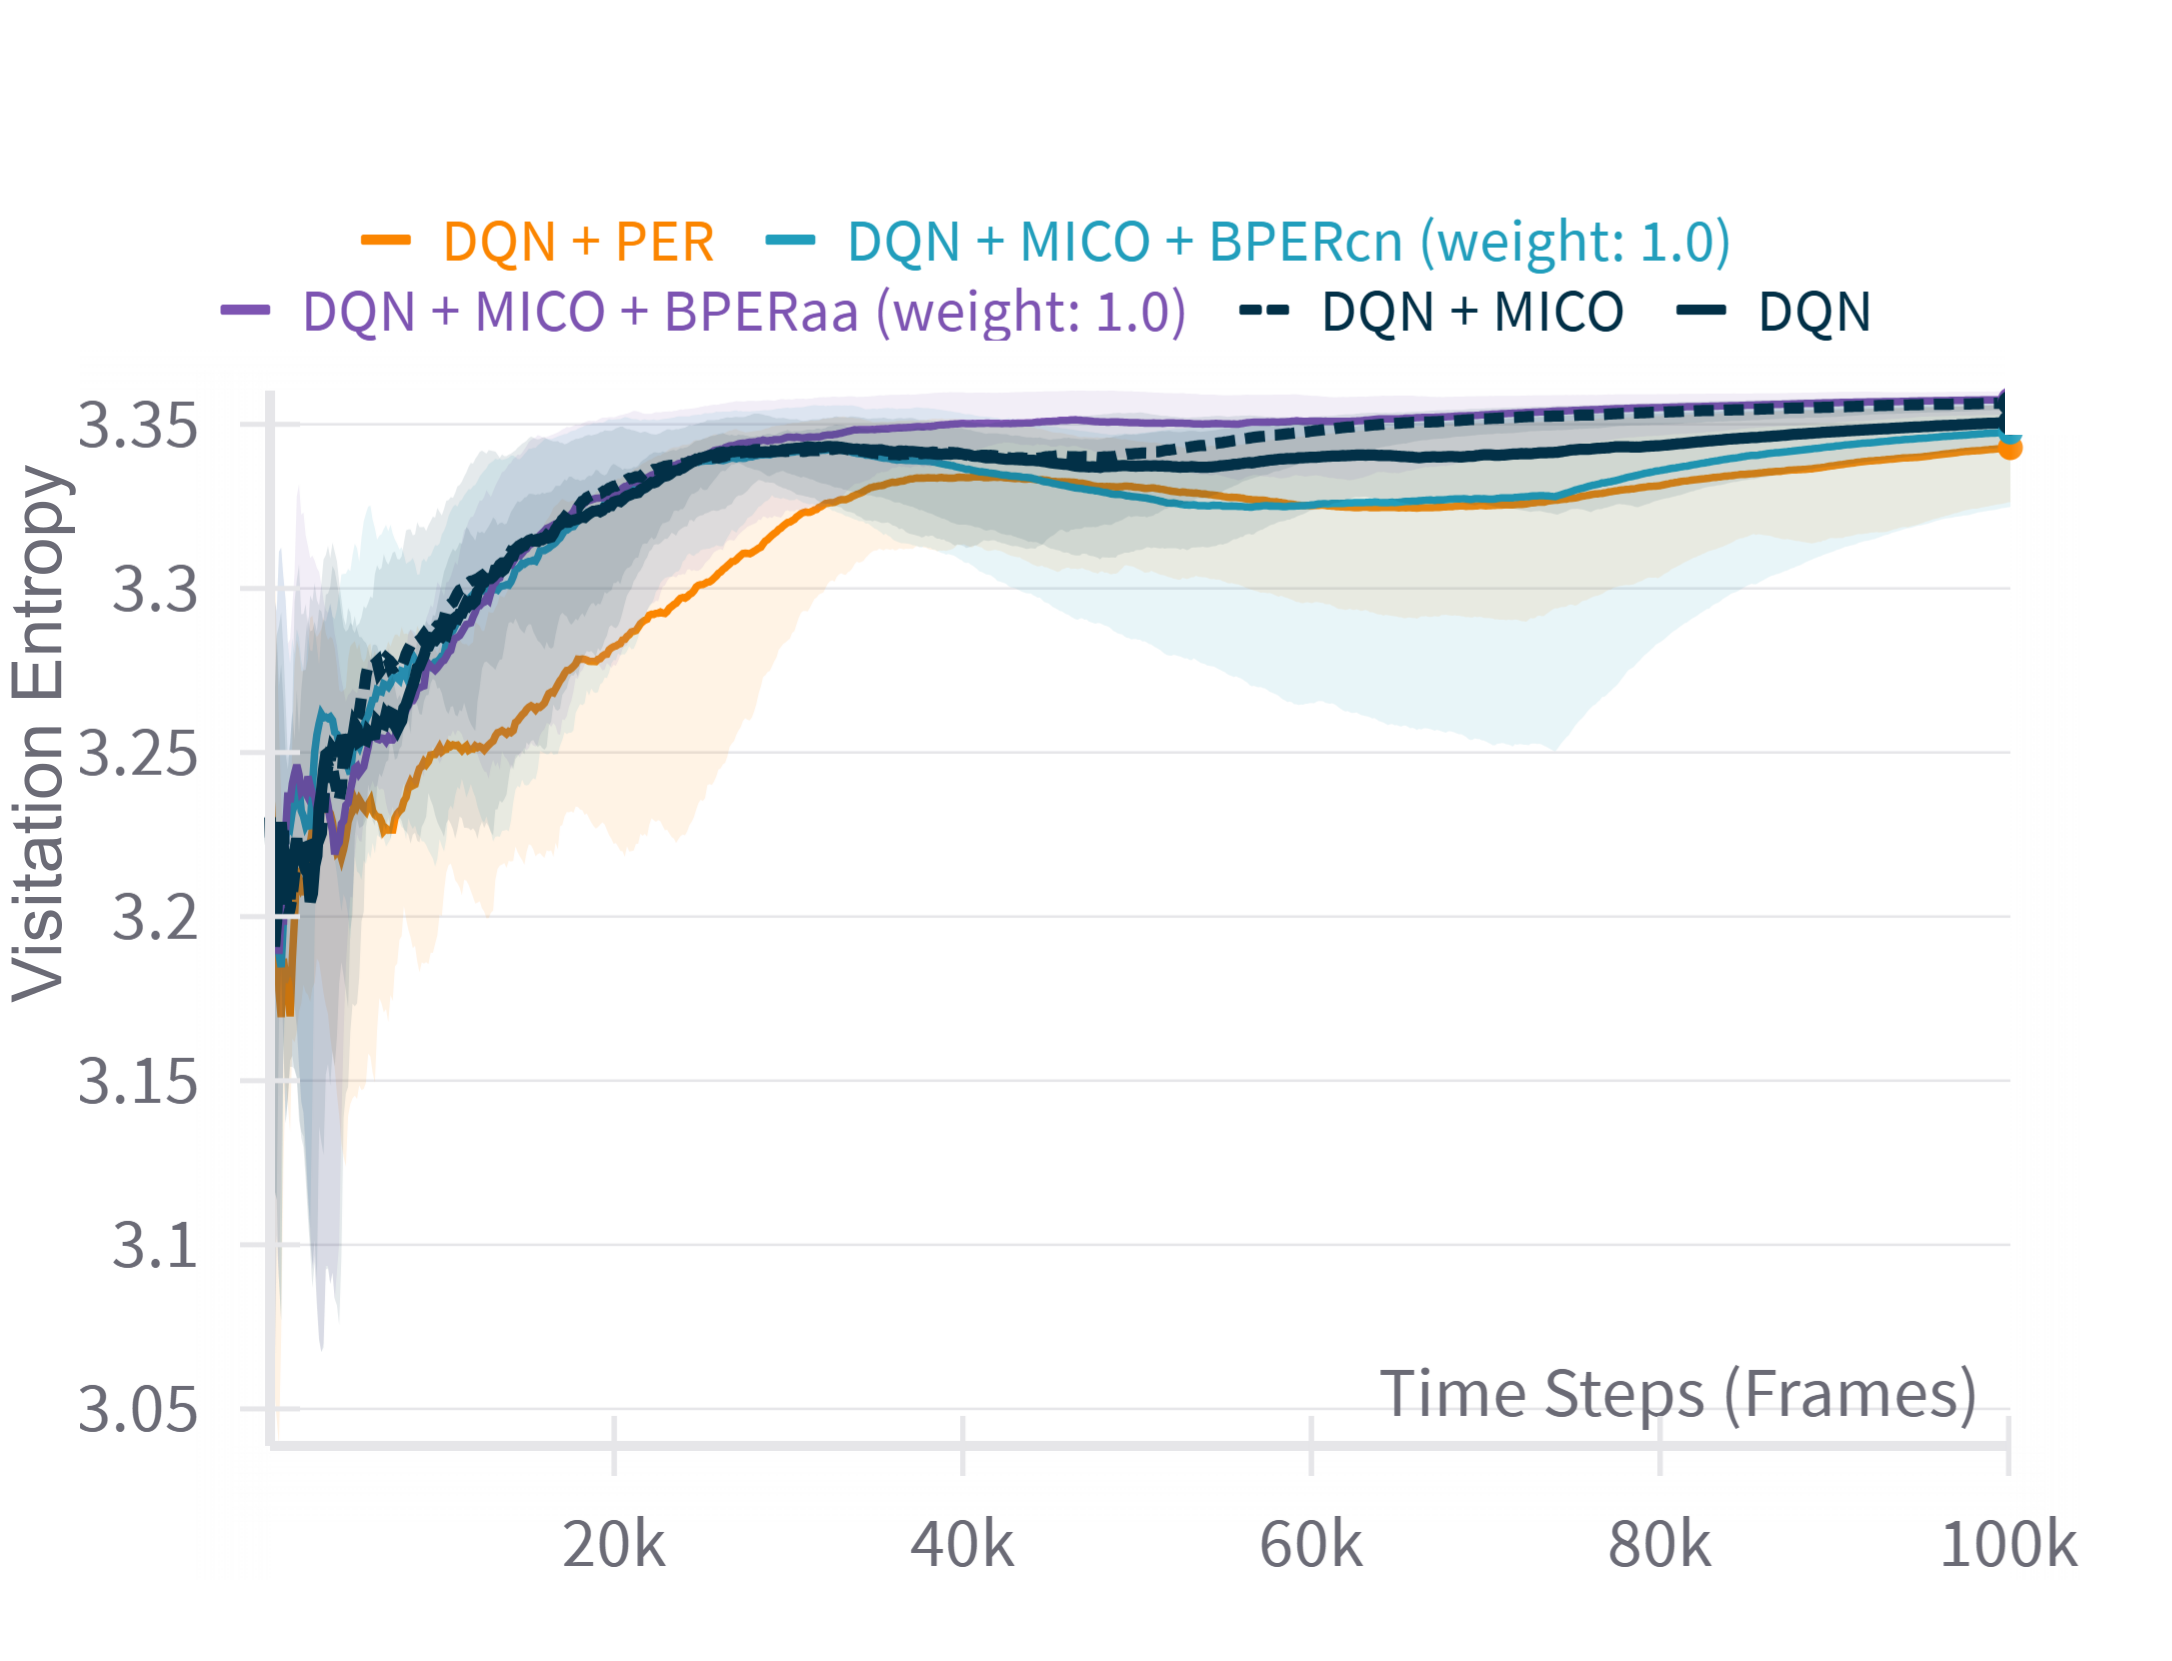
\includegraphics[width=0.7\linewidth]{Results/grid_world/state_visitation_entropy.png}
    \caption{Caption}
    \label{fig:visitation_entropy}
\end{figure}


\section{General RL Performance}

This section aims to explore the capabilities of the proposed method in slightly more complex methods. Figure \ref{fig:episode_reward_more_envs} illustrates the episode reward calculated over a moving average window of 100 episodes in four different environments: MountainCar-v0, LunarLander-v1, CartPole-v1, and Acrobot-v1, averaged over 5 independent executions. The hyperparameter priority weight $\mu$ was set using the best values found\footnote{Note: An exhaustive grid search was not conducted for the priority weight $\mu$. Instead, the values were determined using a trial-and-error approach, where it was observed that when bisimulation is less generally useful, it is better to set smaller values to prioritize more based on TD-error.}, 0.1 for Mountain Car and CartPole, and 1.0 for LunarLander and Acrobot. Please see Appendix \ref{} for experiments with prioritization weights 1.0 for Mountain Car and Cart Pole.

\begin{figure}[h]
    \centering
    \begin{subfigure}{0.45\textwidth}
    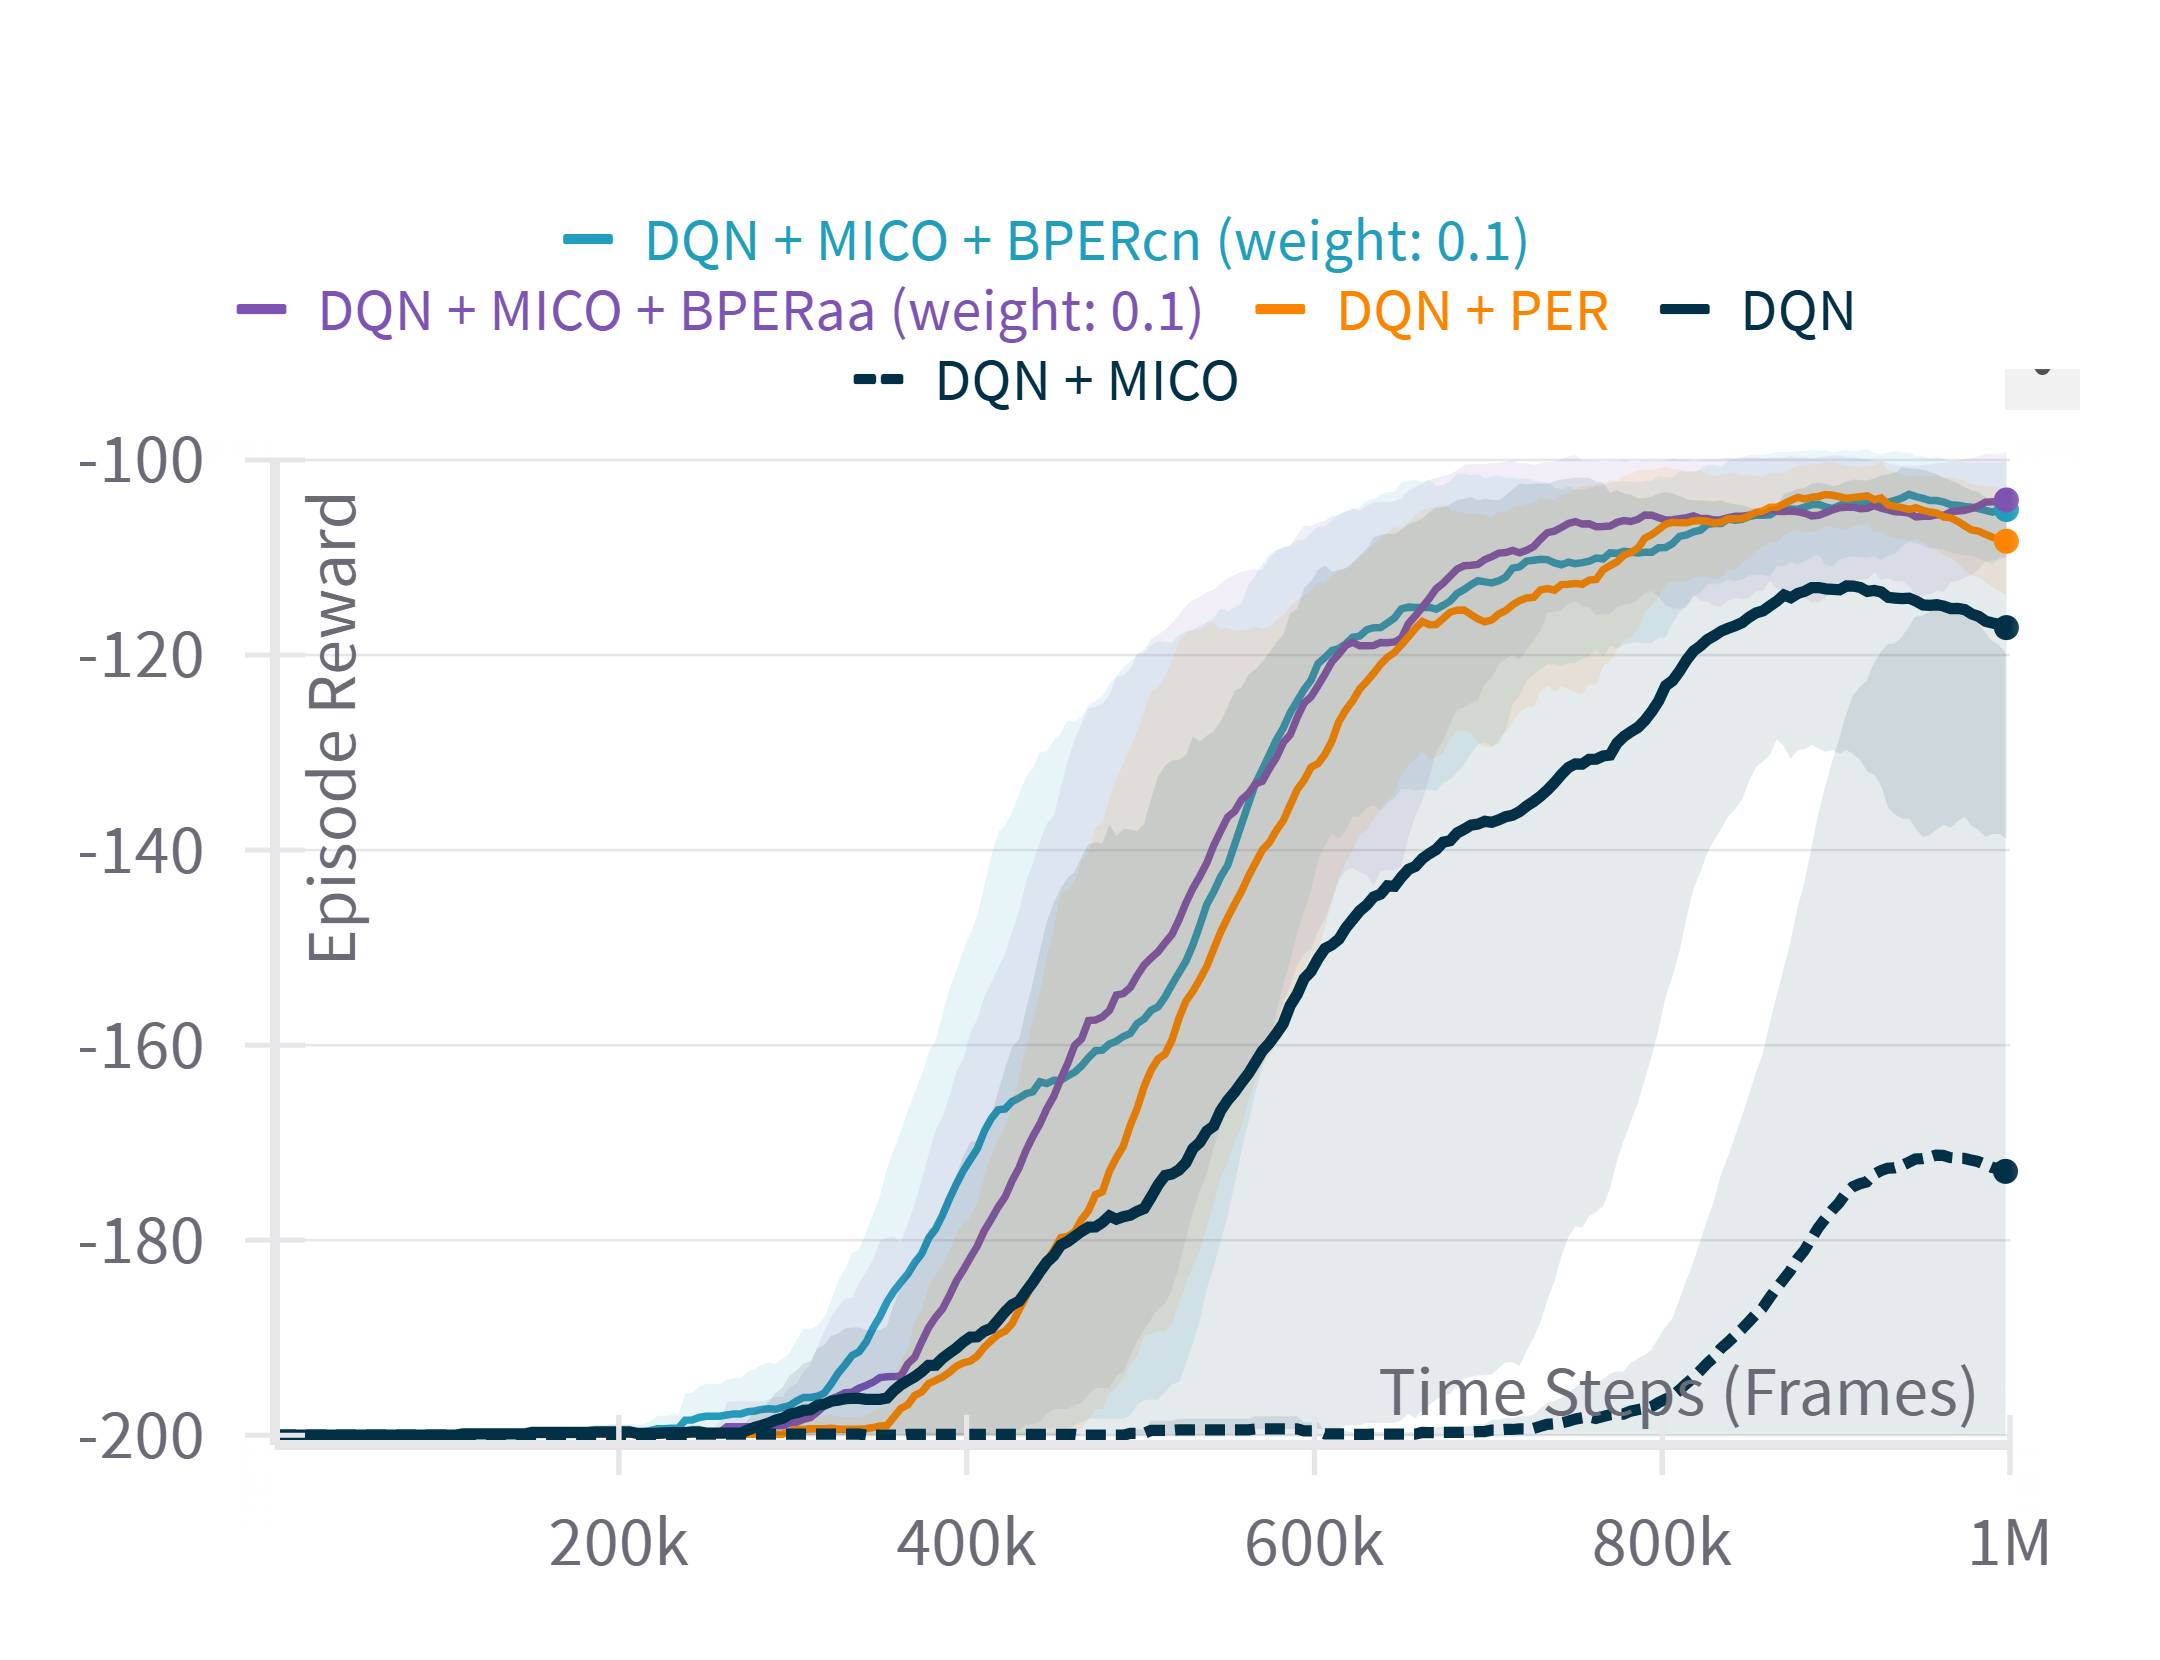
\includegraphics[width=\linewidth]{Results/general_results/episode_reward_mountaincarv0.png}
        \caption{MountainCar-v0}
        \label{fig:episode_reward_mountaincarv0}
    \end{subfigure}
    \hfill
    \begin{subfigure}{0.45\textwidth}
        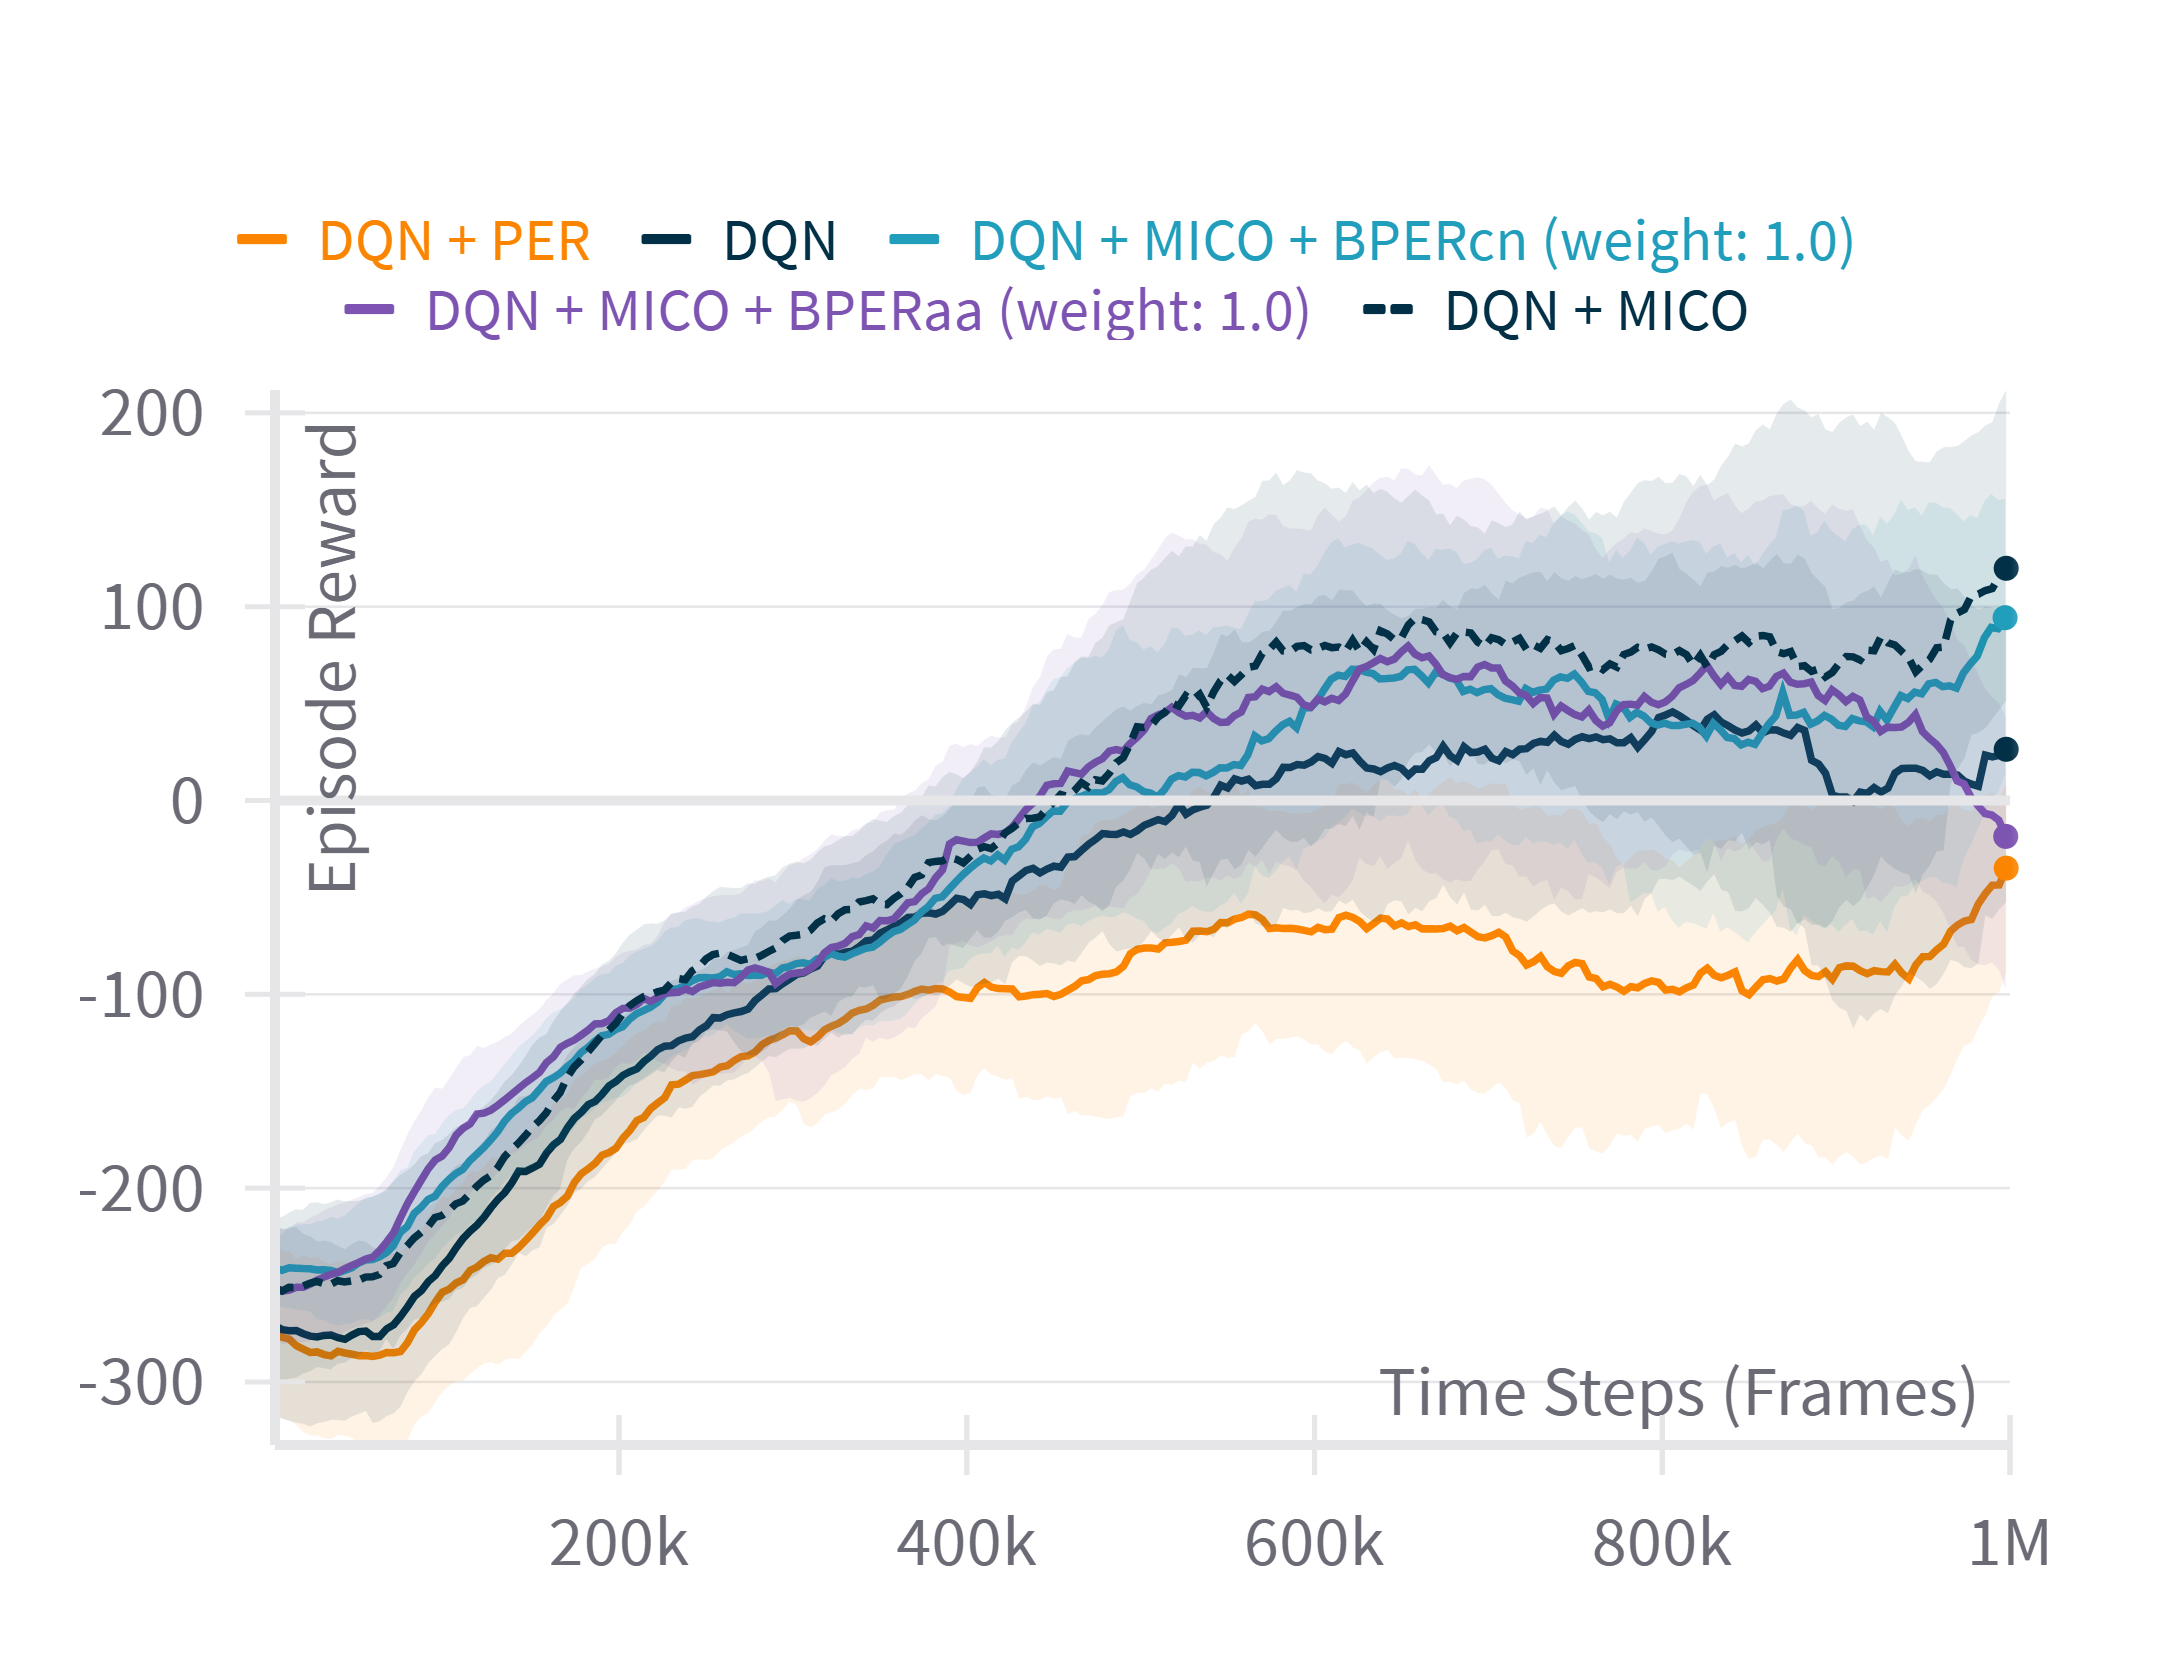
\includegraphics[width=\linewidth]{Results/general_results/episode_reward_lunarlander.png}
        \caption{LunarLander-v1}
        \label{fig:episode_reward_lunarlander}
    \end{subfigure}
    \hfill
    \begin{subfigure}{0.45\textwidth}
        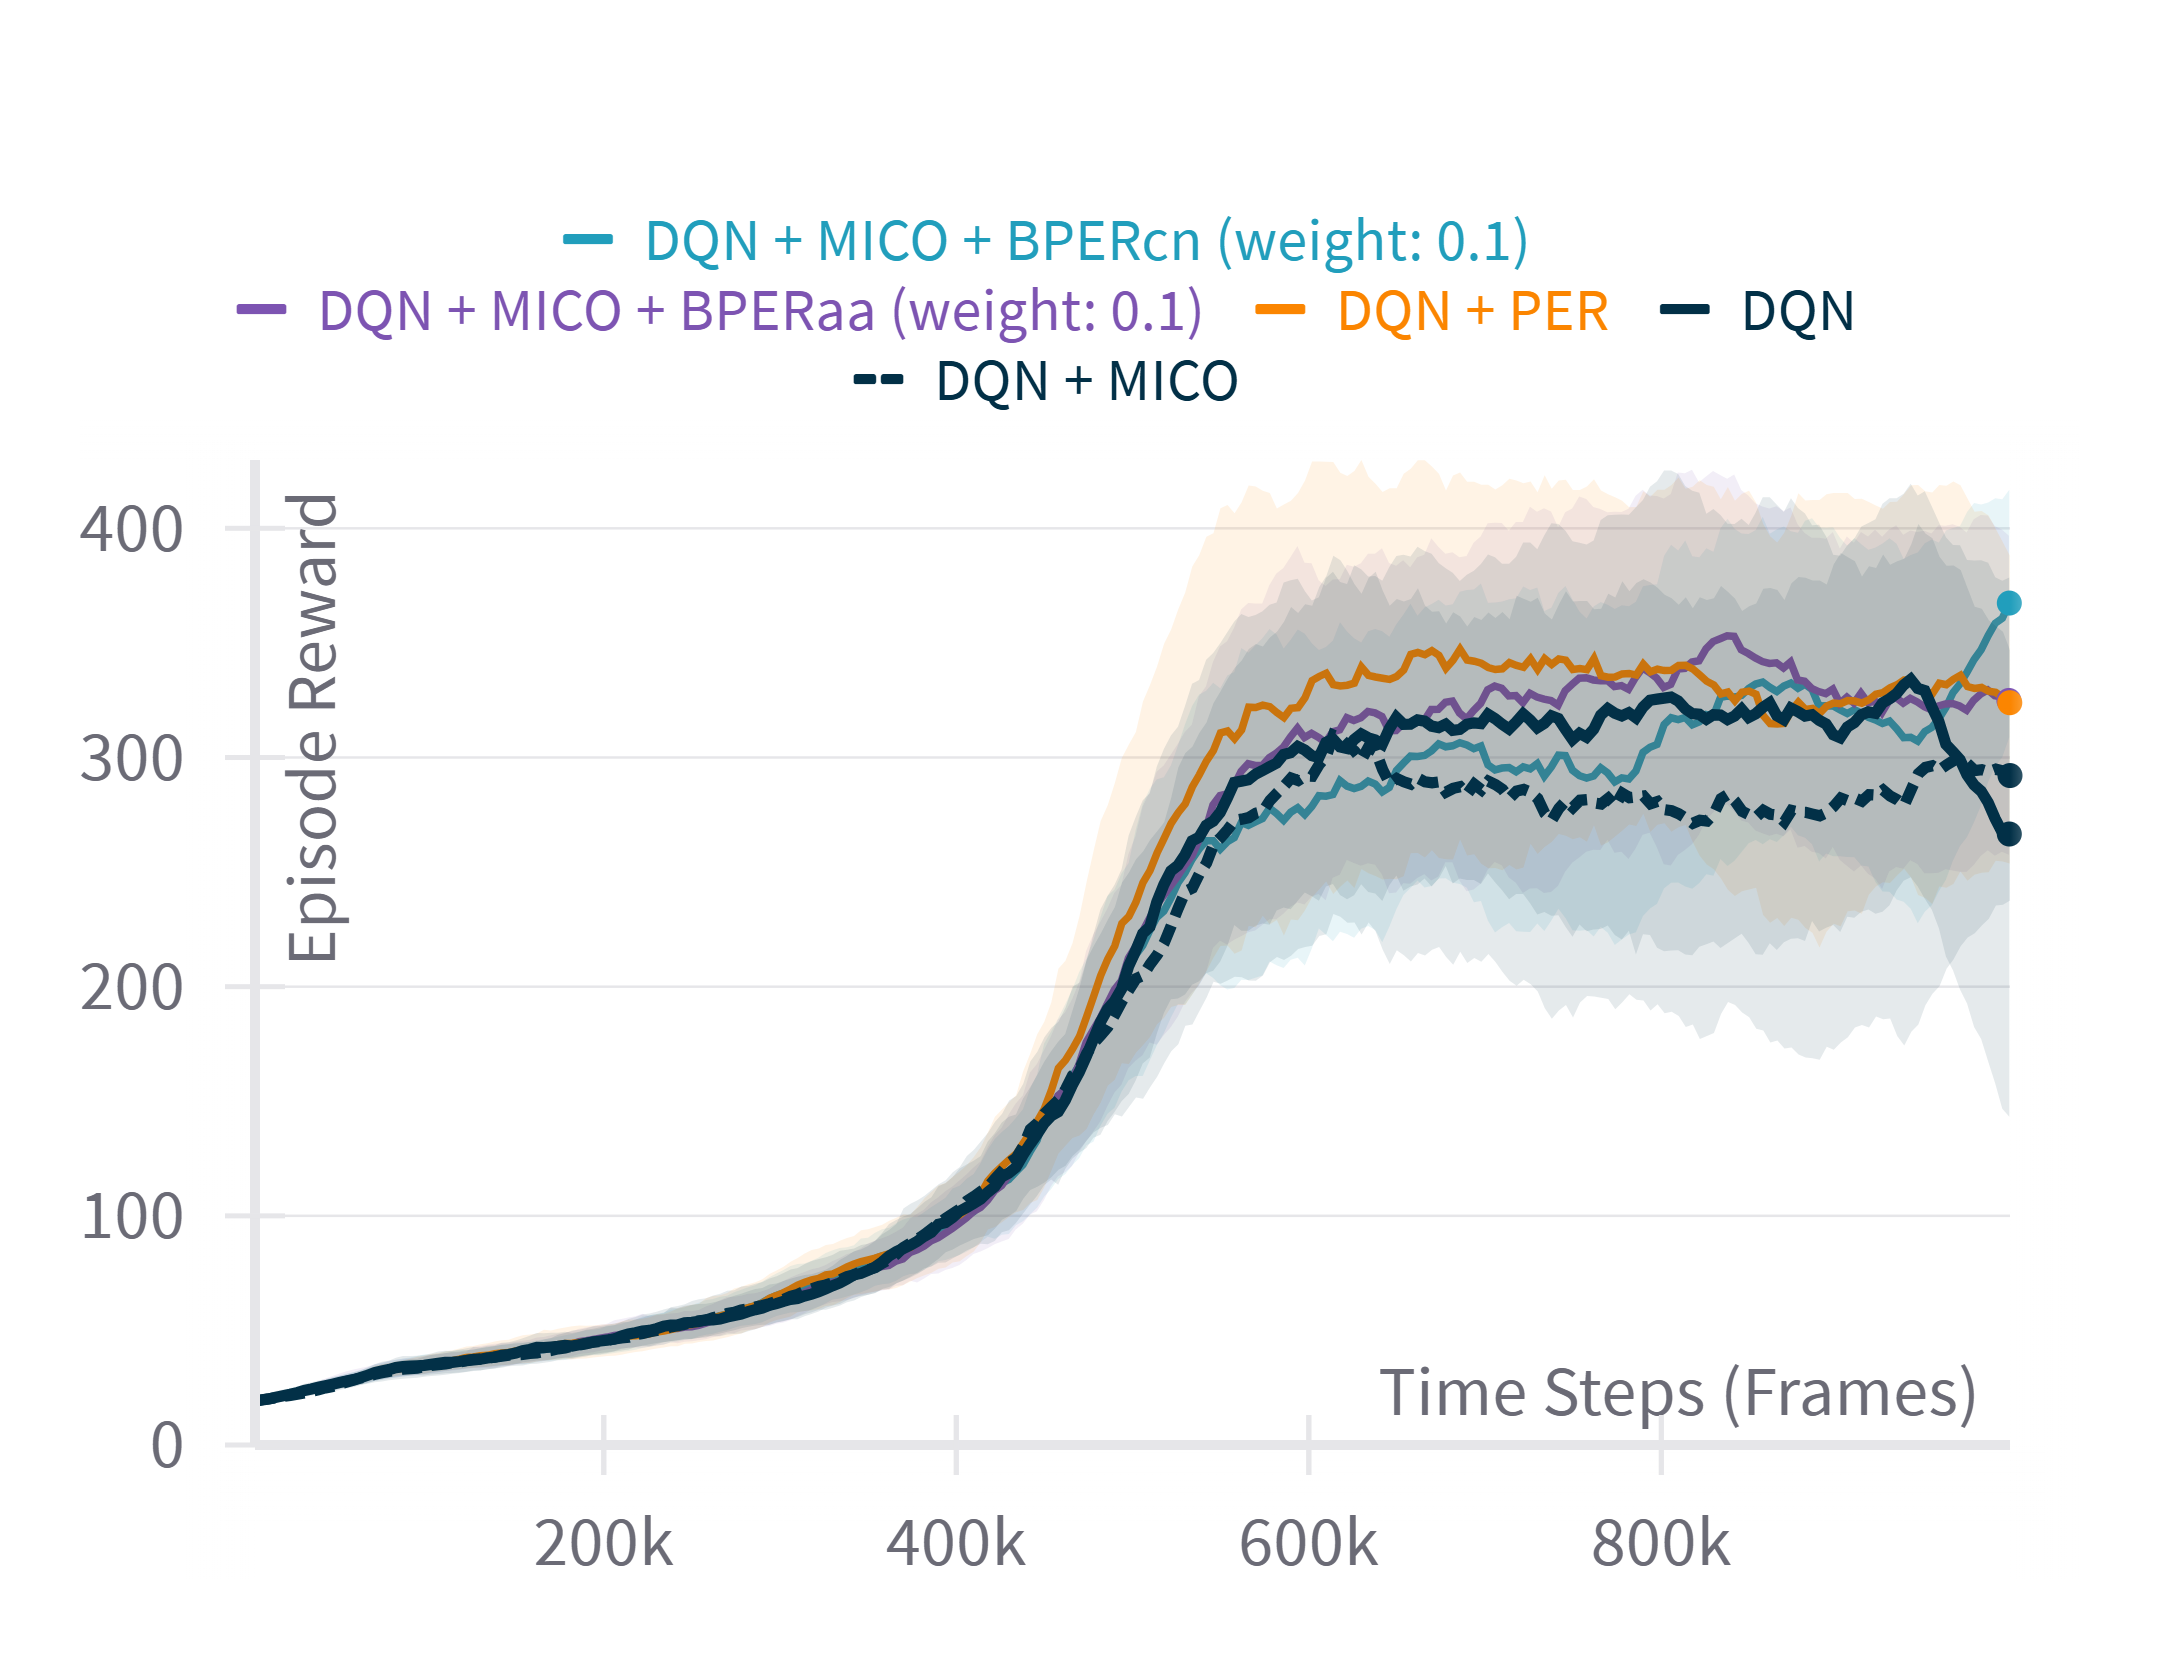
\includegraphics[width=\linewidth]{Results/general_results/episode_reward_cartpolev1.png}
        \caption{CartPole-v1}
        \label{fig:episode_reward_cartpolev1}
    \end{subfigure}
    \hfill
    \begin{subfigure}{0.45\textwidth}
        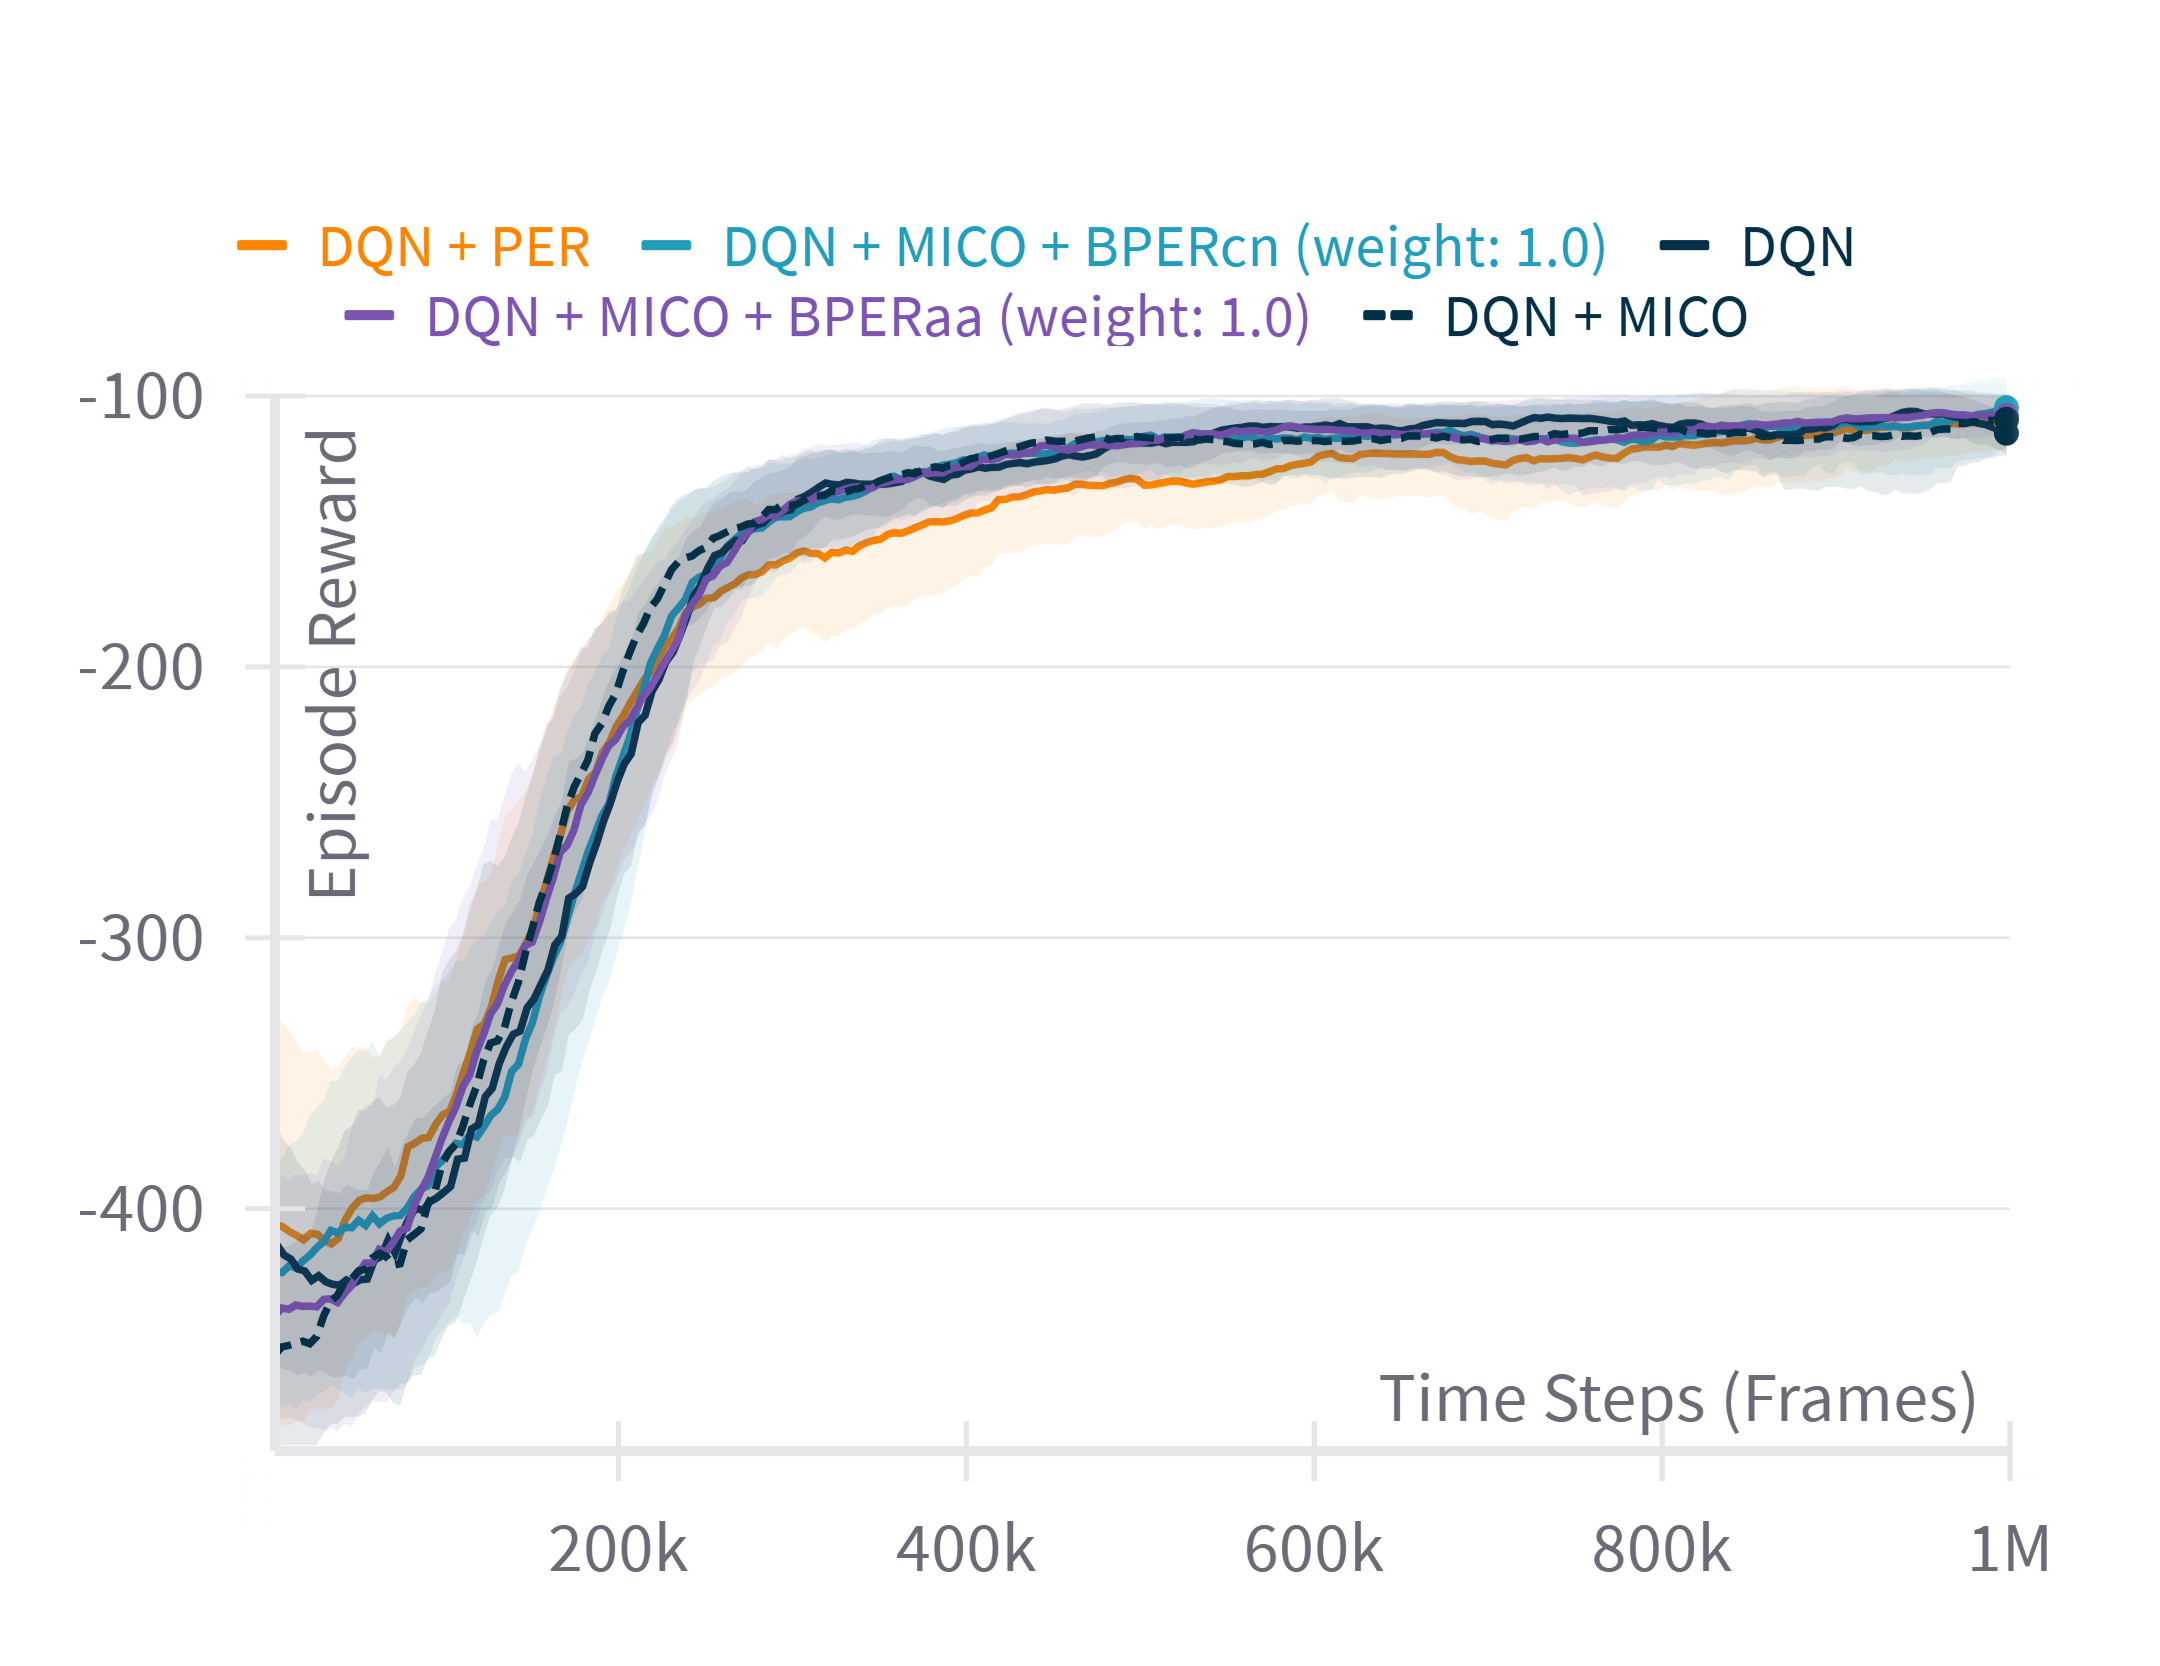
\includegraphics[width=\linewidth]{Results/general_results/episode_reward_acrobotv1.png}
        \caption{Acrobot-v1}
        \label{fig:episode_reward_acrobotv1}
    \end{subfigure}
    \caption{Two images side-by-side}
    \label{fig:episode_reward_more_envs}
\end{figure}

Figure \ref{fig:episode_reward_mountaincarv0} explores the episode reward in the Mountain Car environment, where the bisimulation techniques, BPERcn and BPERaa, outperforms the other methods, with considerable improvements over DQN + MICO baseline. It is important to note that the priority weight is set to 0.1, meaning that most of the prioritization is influenced by the TD-error. This suggests that the bisimulation distance may not be a useful indicator of expected learning progress in this scenario, where the rewards are mostly binary and negative (refer to Appendix \ref{} for results with priority weight 1.0).

Figure \ref{fig:episode_reward_lunarlander} shows the episode reward in the Lunar Lander environment. BPERcn and BPERaa show initially the best performance over all the methods. However, over time, their performance decreases affecting even the learning of the DQN + MICO baseline. Although both strategies outperforms the DQN and DQN + PER methods, the observed benefits appear to derive more from the MICo learning than from the proposed prioritization strategies [Disclaimer\footnote{During our observations, the methods typically outperform the direct baseline DQN + MICo, even when DQN + MICo does not perform better than DQN. However, in this specific instance, a different behavior was observed. Upon revisiting the code and hyperparameter settings, we found a typo where the bisimulation priorities were incorrectly normalized using a logarithmic scale only for this experiment, which could explain the observed issue. These results are provided for reference, but future work should aim to redo this experiment to ensure accuracy.}].

Figure \ref{fig:episode_reward_cartpolev1} shows the episode reward in the CartPole v1 environment. In this scenario, the PER variant is more consistent and outperforms the other methods in most cases. Although the BPERcn and BPERaa alternatives achieve improvements over the direct baseline DQN + MICo, they do not surpass the performance of the DQN baseline. Particularly, DQN + MICo performs worse than DQN, suggesting that in this environment, MICo learning does not provide a clear advantage. This may be due to the difficulty in distinguishing between behaviorally similar or dissimilar states, given the simple reward function (a reward of 1 for each time step) and the limited action space (two actions: left and right). Consequently, it is expected that the BPERcn and BPERaa strategies underperform compared to the other methods. The BPERaa strategy only briefly outperforms the other methods around the 80k time step, but its training is unstable, leading to a subsequent decline in episode reward.

Figure \ref{fig:episode_reward_acrobotv1} shows the episode reward in the Acrobot-v1 environment. In this scenario, BPERcn and BPERaa methods initially demonstrate better performance than the other methods, and they eventually converge to a similar behavior as DQN and DQN + MICo. In contrast, the PER method shows the worst performance over time; even worse than the DQN baseline. Nonetheless, it is important to note that the overlapping results make it challenging to differentiate between the methods; therefore, additional episode reward gains are provided for a clearer analysis bellow.

\begin{figure}[h]
    \centering
    \begin{subfigure}{0.45\textwidth}
    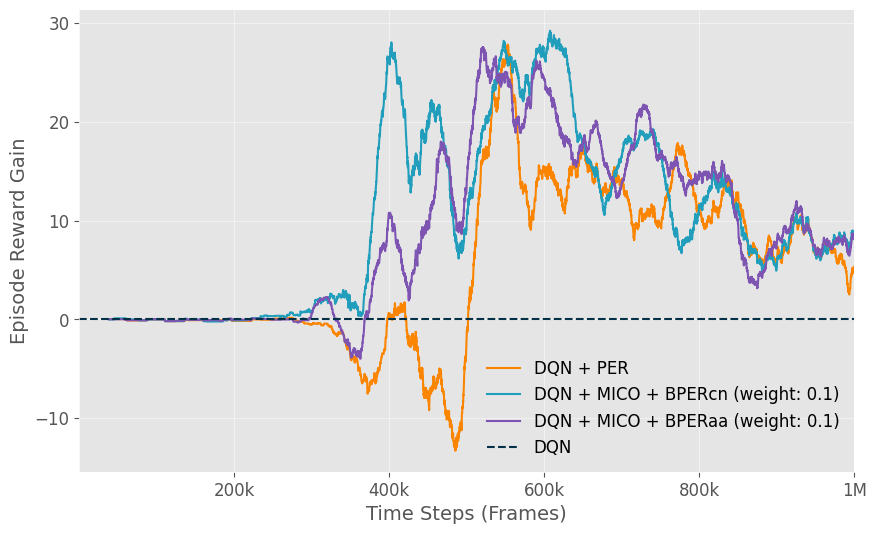
\includegraphics[width=\linewidth]{Results/general_results/mountain_car_reward_gain_vs_dqn.png}
        \caption{MountainCar-v0}
        \label{fig:mountain_car_reward_gain_vs_dqn}
    \end{subfigure}
    \hfill
    \begin{subfigure}{0.45\textwidth}
        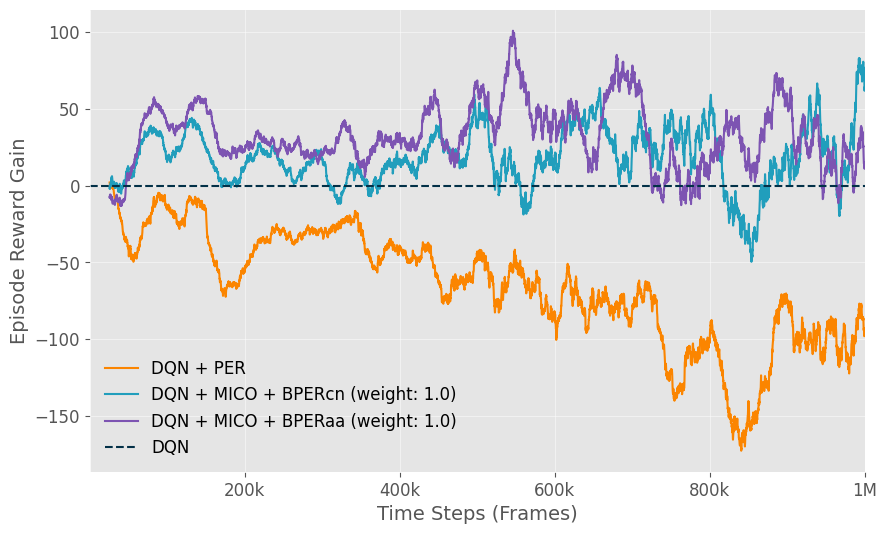
\includegraphics[width=\linewidth]{Results/general_results/lunarlander_reward_gain_vs_dqn.png}
        \caption{LunarLander-v1}
        \label{fig:lunarlander_reward_gain_vs_dqn}
    \end{subfigure}
    \hfill
    \begin{subfigure}{0.45\textwidth}
        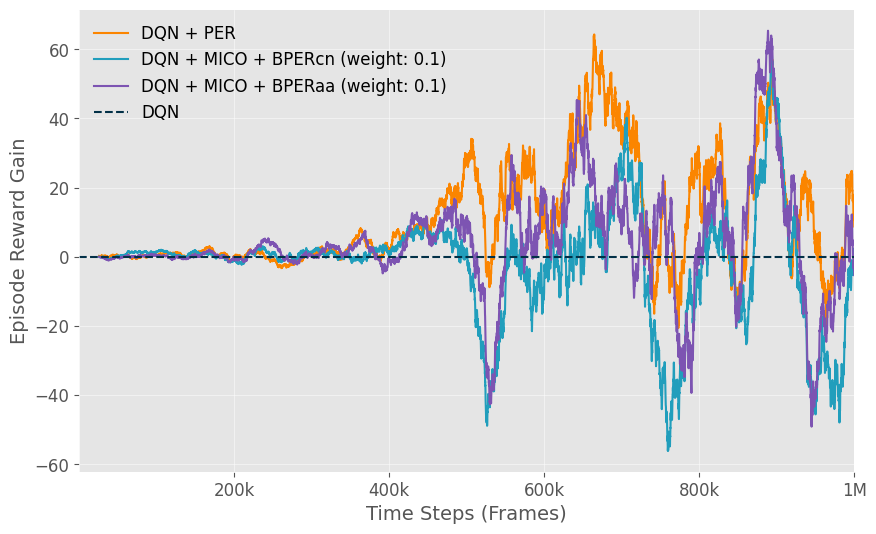
\includegraphics[width=\linewidth]{Results/general_results/cart_polev1_reward_gain_vs_dqn.png}
        \caption{CartPole-v1}
        \label{fig:cart_polev1_reward_gain_vs_dqn}
    \end{subfigure}
    \hfill
    \begin{subfigure}{0.45\textwidth}
        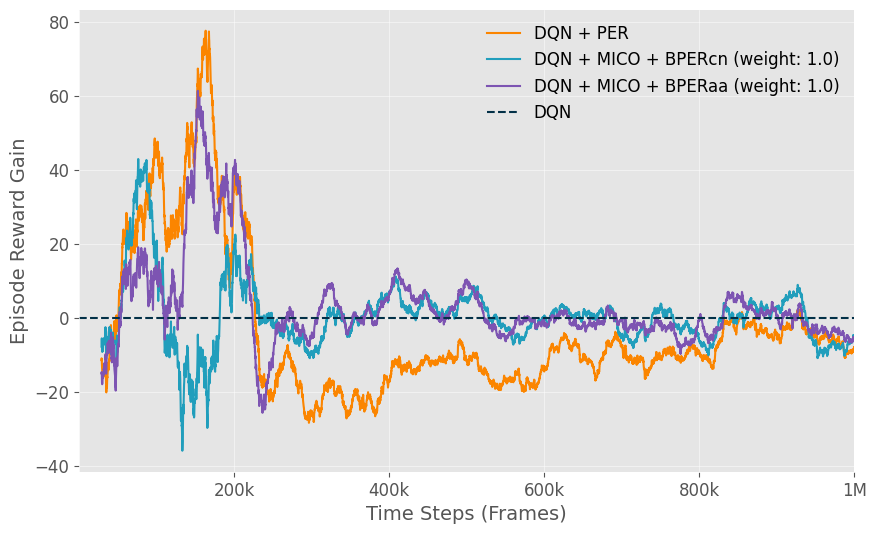
\includegraphics[width=\linewidth]{Results/general_results/acrobotv1_reward_gain_vs_dqn.png}
        \caption{Acrobot-v1}
        \label{fig:acrobotv1_reward_gain_vs_dqn}
    \end{subfigure}
    \caption{Two images side-by-side}
    \label{fig:reward_gain_vs_dqn_methods}
\end{figure}

Figure \ref{fig:reward_gain_vs_dqn_methods} illustrates the episode reward gain relative to the DQN baseline for the three prioritization extensions: PER, BPERcn, and BPERaa, measured in moving average window of 100 episodes, using the equation mentioned in Section \ref{sec:experimental_setup}. r. Notice, in Figure \ref{fig:acrobotv1_reward_gain_vs_dqn}, it is better appreciated the slight improvements of bisimulation strategies over the baseline DQN, which is not possible to observed in episode reward plots. Cartpole v1 results, however, shows a highly variable episode reward gain for our method, BPERcn and BPERaa, and predominant values for the method PER, which is mostly positive over time. An additional evaluation relative to the DQN + MICo baseline is shown for reference in the Appendix \ref{}.

Figure \ref{fig:reward_gain_vs_dqn_methods} illustrates the episode reward gain relative to the DQN baseline for the three prioritization extensions: PER, BPERcn, and BPERaa; measured using a moving average window of 100 episodes, as described in Section \ref{sec:experimental_setup}. Mountain Car, Lunar Lander, and Acrobot-v1 results show that the bisimulation strategies, BPERcn, and BPERaa, obtain mostly positive episode reward gains over time compare to PER alternatives, confirming the findings mentioned earlier. Notice, in Figure \ref{fig:acrobotv1_reward_gain_vs_dqn}, the slight improvements of the bisimulation strategies over the baseline DQN are more clearly observed, which were not evident in the episode reward plots. However, the CartPole-v1 results reveal a highly variable episode reward gain for the BPERcn and BPERaa methods, with predominantly positive values for the PER method over time. An additional evaluation relative to the DQN + MICo baseline is shown for reference in the Appendix \ref{}.

Table \ref{tab:comparison_methods} summarizes the episode reward gains for each method and baseline, presenting the mean and standard deviation over all time steps for each environment. The BPERaa strategy shows the best performance on both the DQN and DQN + MICo baselines in the Acrobot and LunarLander environments, while BPERcn performs best on Mountain Car, and the PER method is most effective on CartPole-v1. It is important to note that the results are highly variable, especially in more complex environments like LunarLander, where the standard deviations reach 185.015 and 191.315 for the DQN and DQN + MICo baselines, respectively. %This indicates significant variability in improvements over time. It is advisable to use another metric to measure the performance, such as the total sum episode reward gain, instead of the mean.

%It may be advisable to use an alternative metric, such as the total sum of episode reward gain, rather than the mean, to measure performance more effectively.





% \begin{table}[h]
%     \centering
%     \caption{Performance Comparison of Different DQN Variants}
%     \label{tab:dqn_comparison}
%     \begin{tabular}{l >{\centering\arraybackslash}p{1.5cm} >{\centering\arraybackslash}p{1.5cm} >{\centering\arraybackslash}p{1.5cm} >{\centering\arraybackslash}p{1.5cm} >{\centering\arraybackslash}p{1.5cm} >{\centering\arraybackslash}p{1.5cm}}
%         \toprule
%                          & \multicolumn{2}{c}{\textbf{PER}}                       & \multicolumn{2}{c}{\textbf{BPERcn}}            & \multicolumn{2}{c}{\textbf{BPERaa}}             \\
%                          & {\color[HTML]{656565} \footnotesize DQN} & {\color[HTML]{656565} \footnotesize MICO} & {\color[HTML]{656565} \footnotesize DQN} & {\color[HTML]{656565} \footnotesize MICO} & {\color[HTML]{656565} \footnotesize DQN} & {\color[HTML]{656565} \footnotesize MICO} \\
%         \midrule
%         \textbf{MountainCar-v0} & $5.344 \pm 21.016$ & $39.088 \pm 39.151$   & $\mathbf{10.145} \pm \mathbf{21.471} $    & $\mathbf{43.889} \pm \mathbf{38.863}$  & $9.021 \pm 19.756$   & $42.765 \pm 39.060$     \\
%         \textbf{Cartpole-v1}    & $\mathbf{10.975} \pm \mathbf{133.140}$    & $\mathbf{24.23} \pm \mathbf{135.122}$   & $-2.100 \pm 134.322$   & $11.648 \pm 129.970$  & $3.790 \pm 134.959$    & $17.539 \pm 134.593$     \\
%         \textbf{Acrobot-v1}     & $-3.279 \pm 79.455$  & $-6.878 \pm 74.916$   & $0.250 \pm 78.057$    & $-3.350 \pm 73.122$  & $\mathbf{2.915} \pm \mathbf{75.618}$    & $\mathbf{-0.685} \pm \mathbf{70.853}$     \\
%         \textbf{LunarLander-v1} & $-65.620 \pm 175.613$    & $-107.075 \pm 183.781$   & $18.800 \pm 191.309$    & $-22.654 \pm 194.957$  & $\mathbf{32.125} \pm \mathbf{185.015}$    & $\mathbf{-9.330} \pm \mathbf{191.315}$   \\
%         \bottomrule
%     \end{tabular}
% \end{table}


\begin{table}[h]
    \hspace*{-1cm}
    \setlength{\tabcolsep}{2.5pt}
    \centering
    \begin{tabular}{llcccc}
        \toprule
        & \textbf{Baseline} & \textbf{MountainCar-v0} & \textbf{Cartpole-v1} & \textbf{Acrobot-v1} & \textbf{LunarLander-v1} \\
        \midrule
        {\footnotesize\textbf{PER}} & {\footnotesize\textbf{DQN}} & $5.344 \pm 21.016$ & $\mathbf{10.975} \pm \mathbf{133.140}$ & $-3.279 \pm 79.455$ & $-65.620 \pm 175.613$ \\
         & {\footnotesize\textbf{MICO}} & $39.088 \pm 39.151$ & $\mathbf{24.23} \pm \mathbf{135.122}$ & $-6.878 \pm 74.916$ & $-107.075 \pm 183.781$ \\
        {\footnotesize\textbf{BPERcn}} & {\footnotesize\textbf{DQN}} & $\mathbf{10.145} \pm \mathbf{21.471}$ & $-2.100 \pm 134.322$ & $0.250 \pm 78.057$ & $18.800 \pm 191.309$ \\
        & {\footnotesize\textbf{MICO}} & $\mathbf{43.889} \pm \mathbf{38.863}$ & $11.648 \pm 129.970$ & $-3.350 \pm 73.122$ & $-22.654 \pm 194.957$ \\
        {\footnotesize\textbf{BPERaa}} & {\footnotesize\textbf{DQN}} & $9.021 \pm 19.756$ & $3.790 \pm 134.959$ & $\mathbf{2.915} \pm \mathbf{75.618}$ & $\mathbf{32.125} \pm \mathbf{185.015}$ \\
        & {\footnotesize\textbf{MICO}} & $42.765 \pm 39.060$ & $17.539 \pm 134.593$ & $\mathbf{-0.685} \pm \mathbf{70.853}$ & $\mathbf{-9.330} \pm \mathbf{191.315}$ \\
        \bottomrule
    \end{tabular}
    \caption{Performance Comparison of Different DQN Variants}
    \label{tab:comparison_methods}
\end{table}

\subsection{Mean Batch Priority}

% The increasing complexity of environments makes difficult to calculate prioritization distributions for a better detail evaluation; it is impractical to measure bisimulation distributions in a large experience replay with high-dimensional stacked states. However, it is still possible to have a glimpse appreciation of the priority values by studying the average priority in each minibatch sampled during training. Specifically, Figure \ref{fig:log_mean_batch_priority_methods} illustrates the log mean batch priority per method over time, averaged over 5 independent executions. Notice the log scale was used to compare the methods because bisimulation distances and td-errors could vary by some orders of magnitude, and both can reach large values over time. In all environments, the BPERcn and BPERaa methods consistently have large priority values on average than the PER method. This result have different interpretations: (1) a large value could indicate an efficient prioritization because the algorithmn over the sampled mini-batches will contain experiences with high priorities values effectively increasing the average priority in the mini batch over time, (2) a large value could indicate a saturated case scenario, where only few priorities are highly prioritized over the others avoiding a correct diversity in data. 

% According to the previous results in episode reward, it seems to be a mix of both depending the case. For examples, in environments such as LunarLander and Mountain and Acrobot although initially present a increasing episode reward over time the reward is reduced a bit reaching similar results to DNQ + MICO, indicating that the algorithm is following in the second scenario. However, results from Mountain Car and Cart Pole indicate an increasing performance over the DQN + MICo baseline; falling in the first scenaro\footnote{Notice even in the cases with priority weight 1.0. This increasing behavior over DQN + MICo is presented even if in those scanario MICO learning does not increase the DQN performance.}.

The increasing complexity of environments makes it difficult to calculate prioritization distributions for a more detailed evaluation; it is impractical to measure bisimulation distributions in a large experience replay with high-dimensional stacked states. However, it is still possible to gain some insight into the priority values by studying the average priority in each minibatch sampled during training. Figure \ref{fig:log_mean_batch_priority_methods} illustrates the log mean batch priority per method over time, averaged over 5 independent executions. A logarithmic scale was used to compare the methods because bisimulation distances and TD-errors can vary by several orders of magnitude, and both can reach large values over time. In all environments, the BPERcn and BPERaa methods consistently exhibit higher average priority values compared to the PER method.

This result can be interpreted in two ways: (1) A high average priority value might indicate efficient prioritization, where the sampled minibatches contain experiences with high priority values, effectively increasing the average priority over time; (2) A high average priority value could also suggest a saturated scenario, where only a few experiences are highly prioritized, potentially reducing diversity in the data. According to the previous results for episode reward in Figure \ref{fig:episode_reward_more_envs}, both interpretations seem relevant depending on the environment. For example, in the LunarLander environment, although there is an initial increase in episode reward, performance eventually declines to levels similar to DQN + MICo, suggesting that the algorithm is likely falling into the second scenario. Conversely, results from Mountain Car, Acrobot, and CartPole indicate sustained performance improvements over the DQN + MICo baseline, aligning with the first scenario\footnote{Note this improvement over DQN + MICo is observed even with a priority weight of 1.0, where, although MICo learning does not enhance DQN performance, the BPERaa and BPERcn methods still outperform DQN + MICo.}.

\begin{figure}[h]
    \centering
    \begin{subfigure}{0.45\textwidth}
    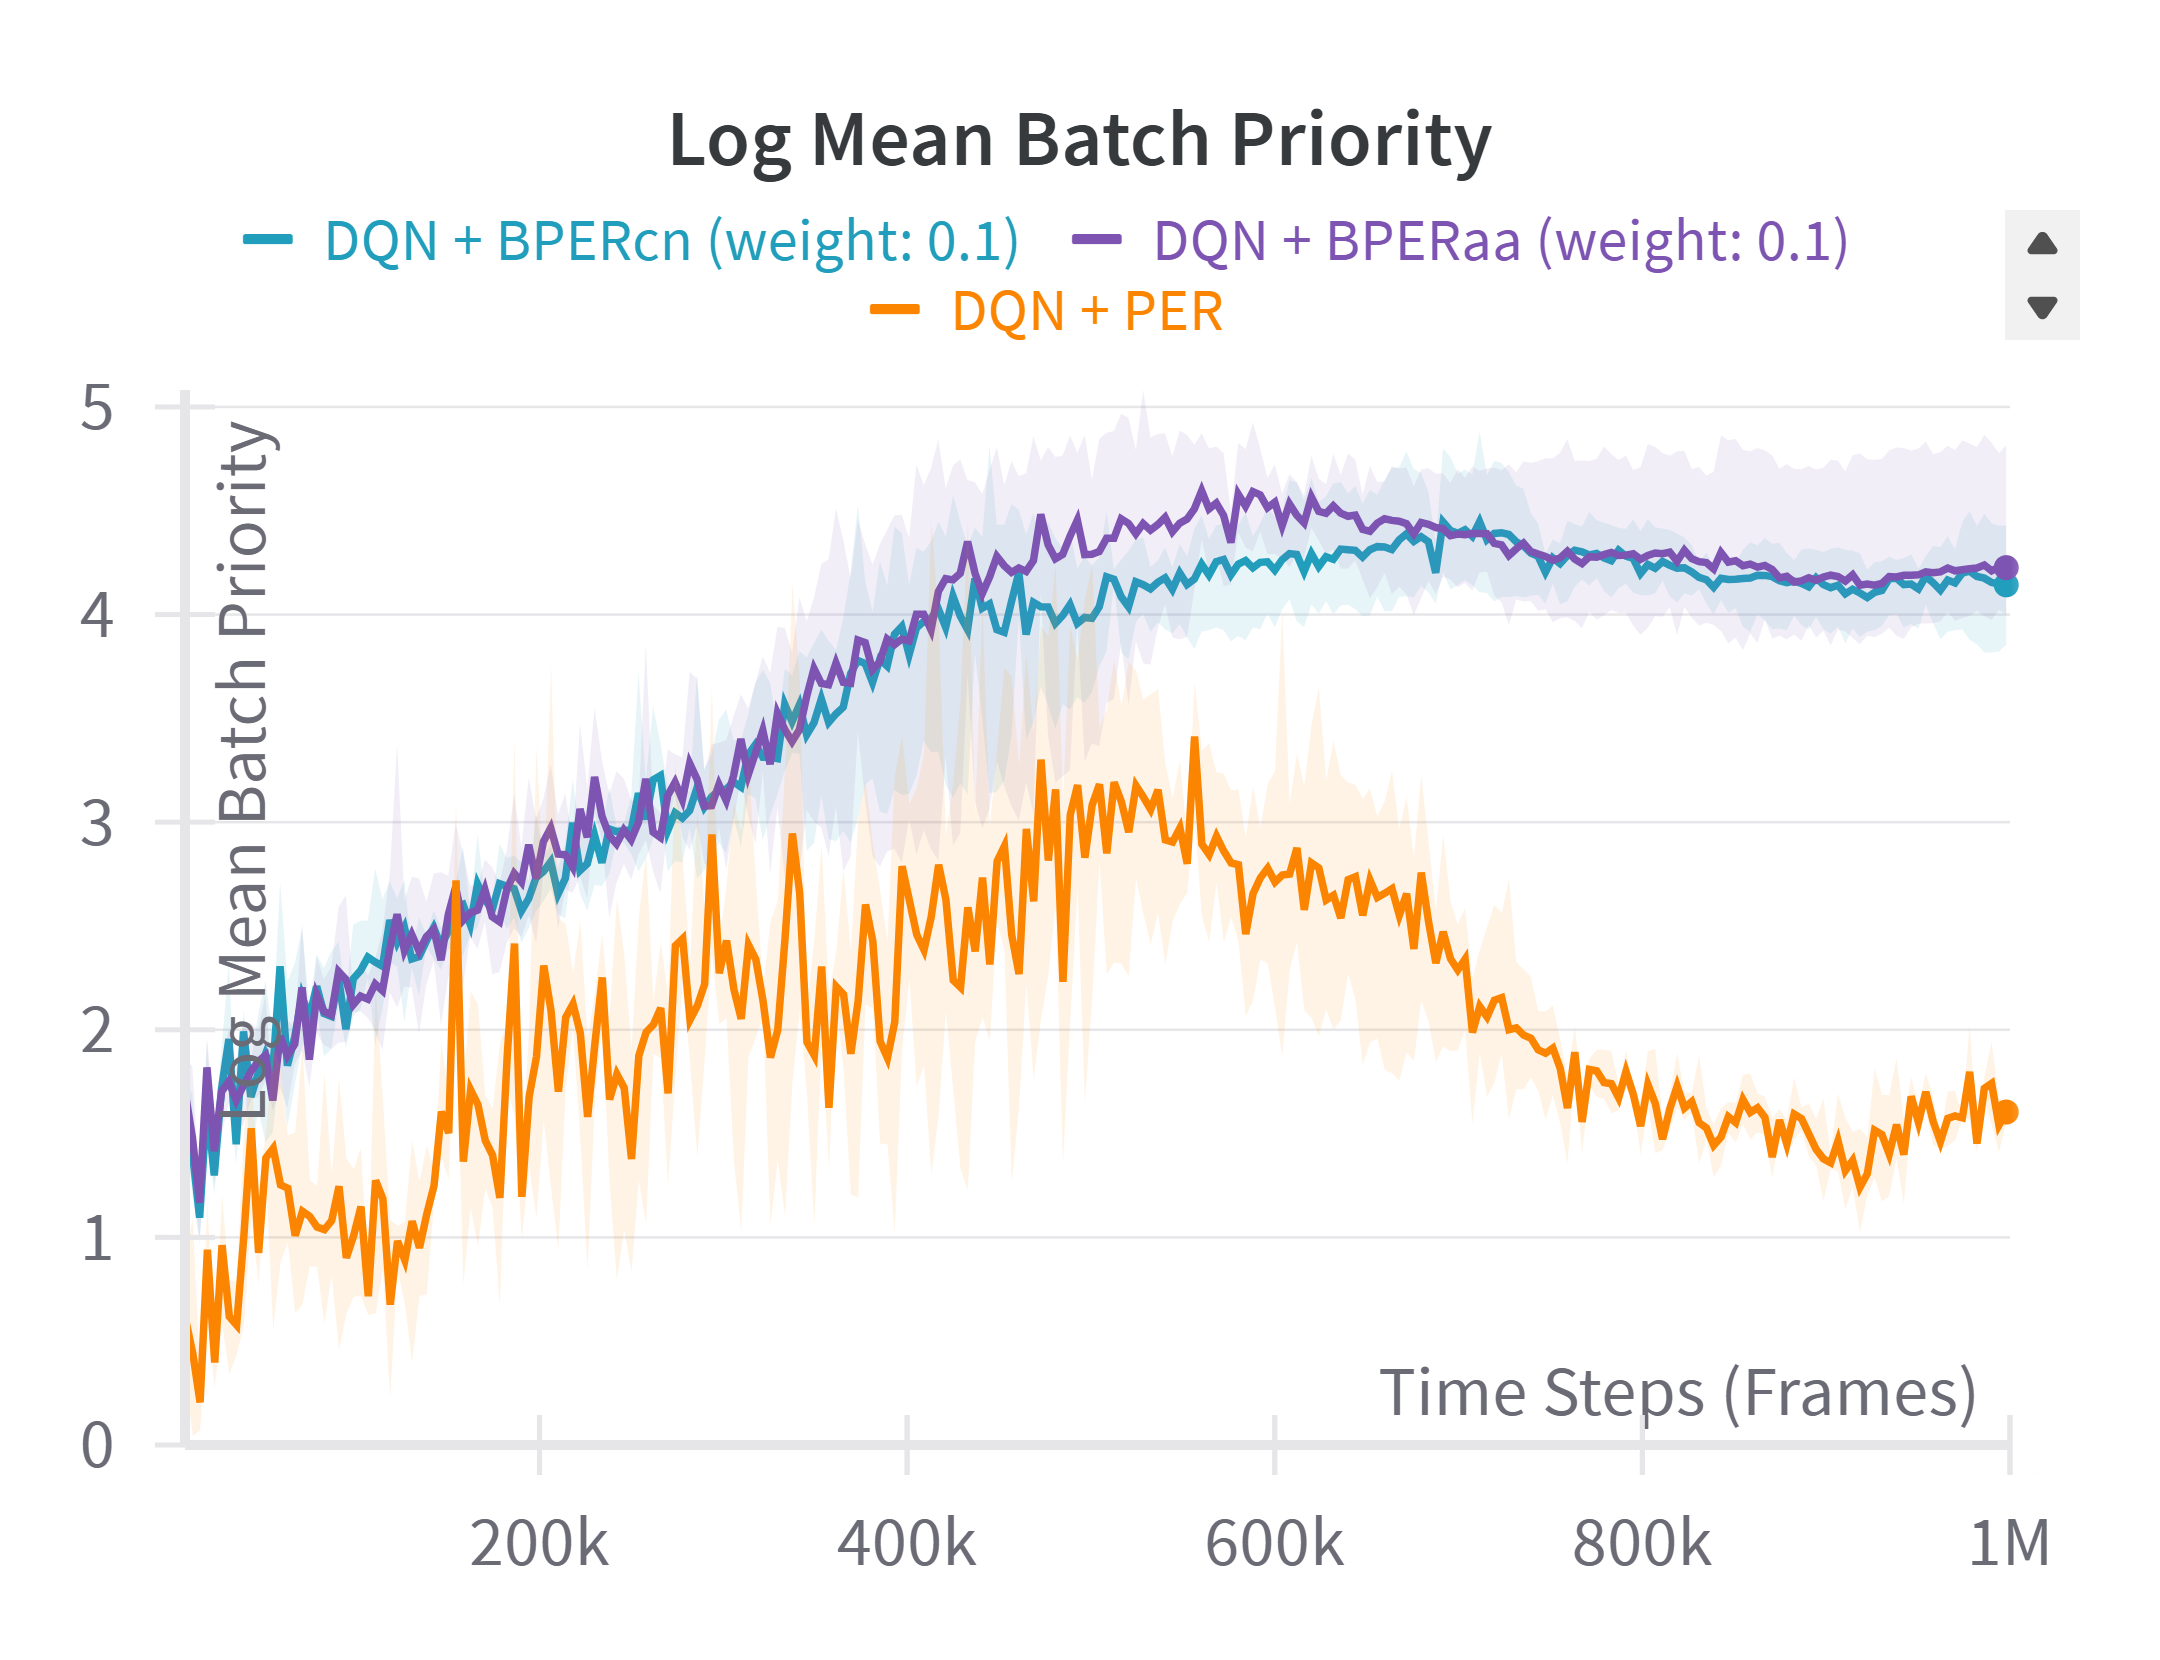
\includegraphics[width=\linewidth]{Results/general_results/log_mean_batch_priority_mountain_car.png}
        \caption{MountainCar-v0}
        \label{fig:log_mean_batch_priority_mountain_car}
    \end{subfigure}
    \hfill
    \begin{subfigure}{0.45\textwidth}
        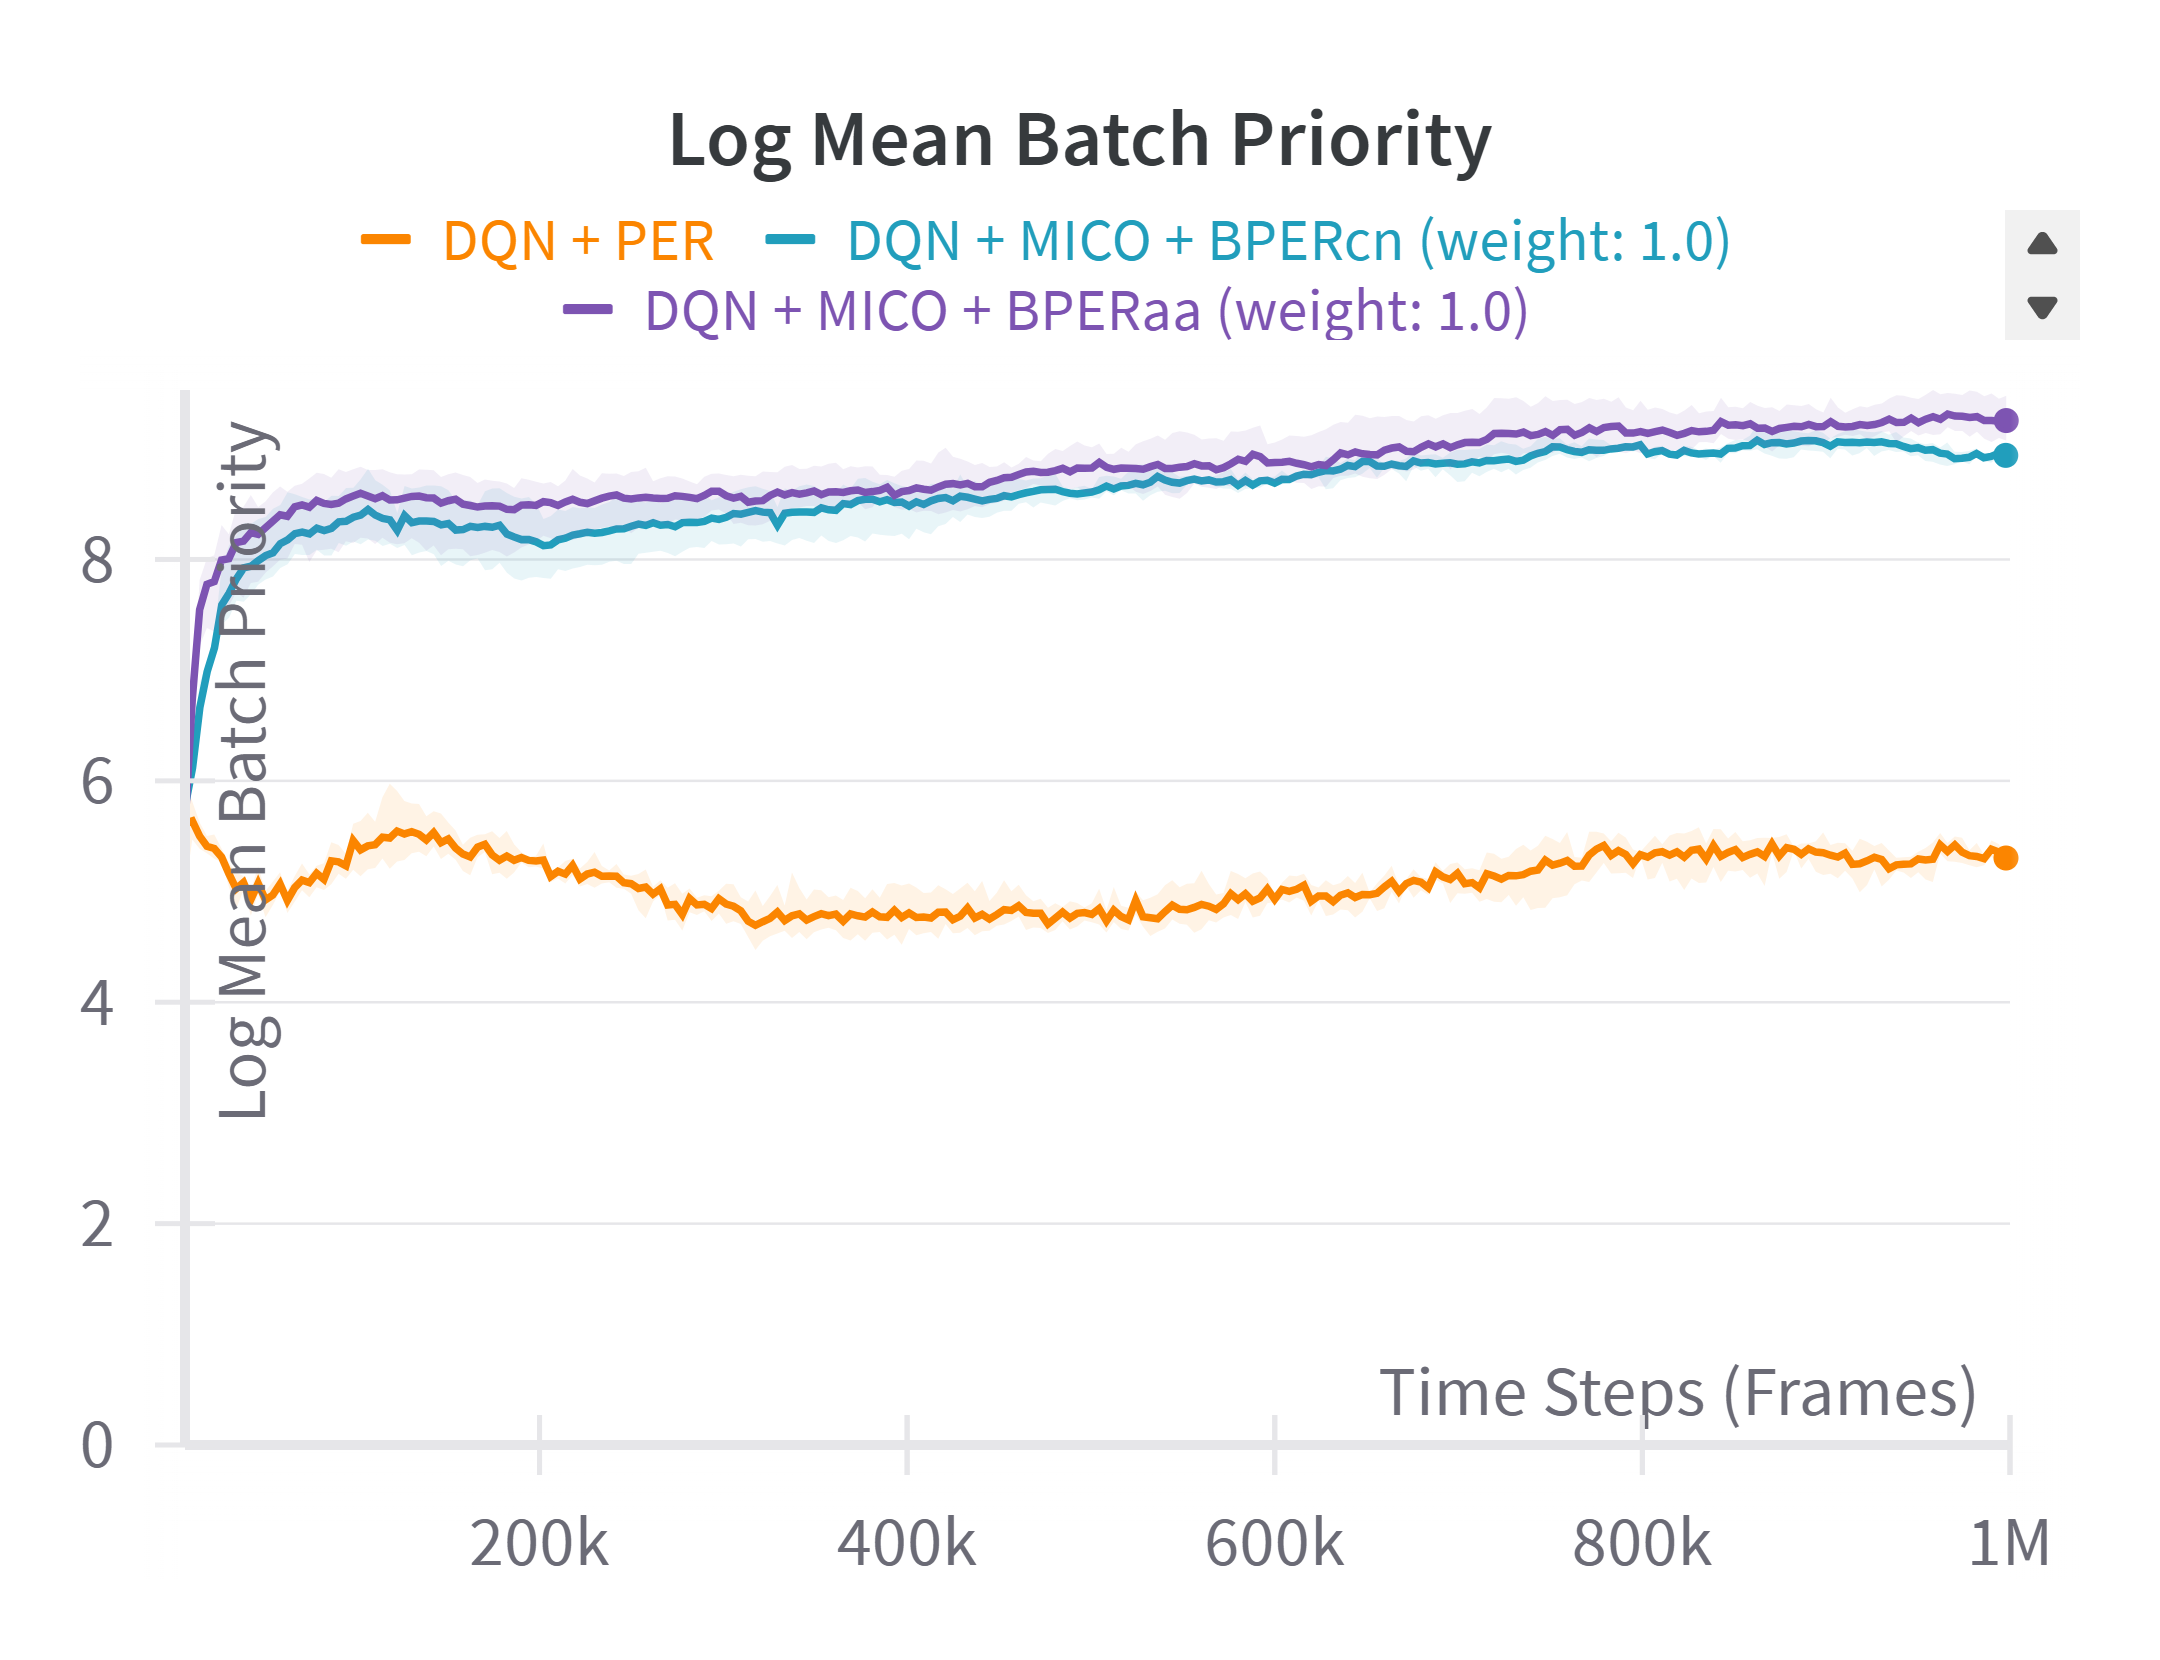
\includegraphics[width=\linewidth]{Results/general_results/log_mean_batch_priority_lunarlander.png}
        \caption{LunarLander-v1}
        \label{fig:log_mean_batch_priority_lunarlander}
    \end{subfigure}
    \hfill
    \begin{subfigure}{0.45\textwidth}
        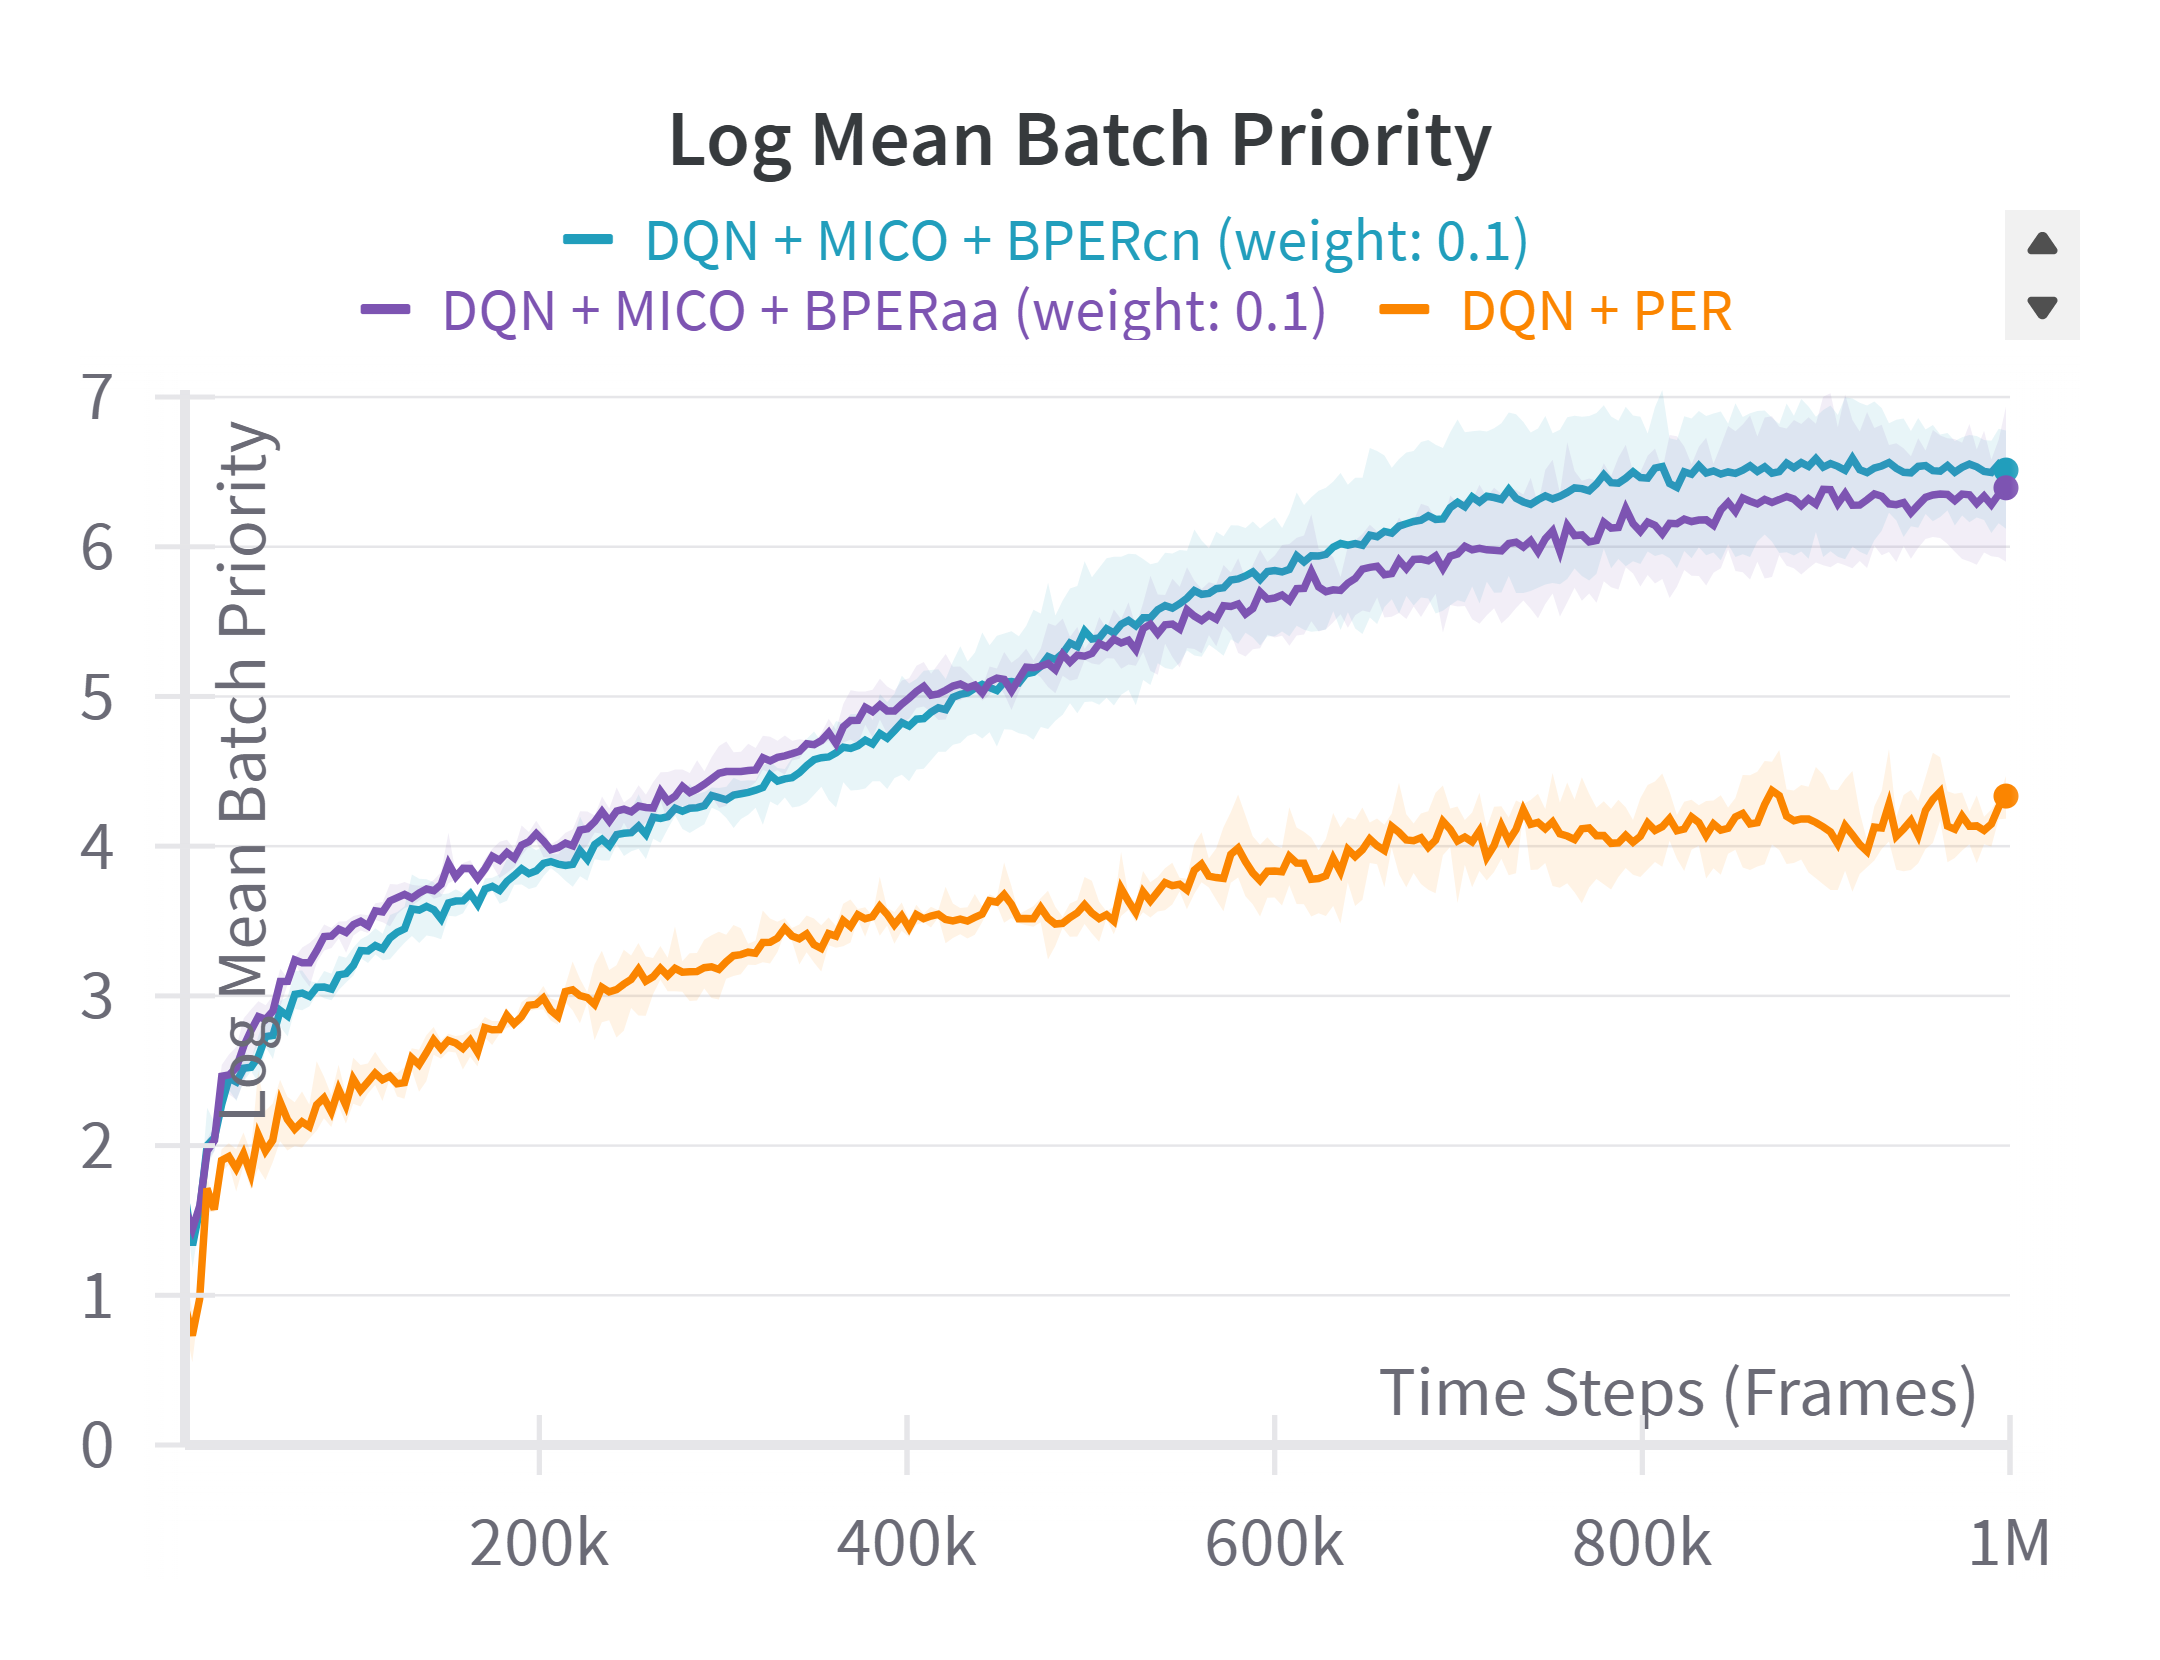
\includegraphics[width=\linewidth]{Results/general_results/log_mean_batch_priority_cartpolev1.png}
        \caption{CartPole-v1}
        \label{fig:log_mean_batch_priority_cartpolev1}
    \end{subfigure}
    \hfill
    \begin{subfigure}{0.45\textwidth}
        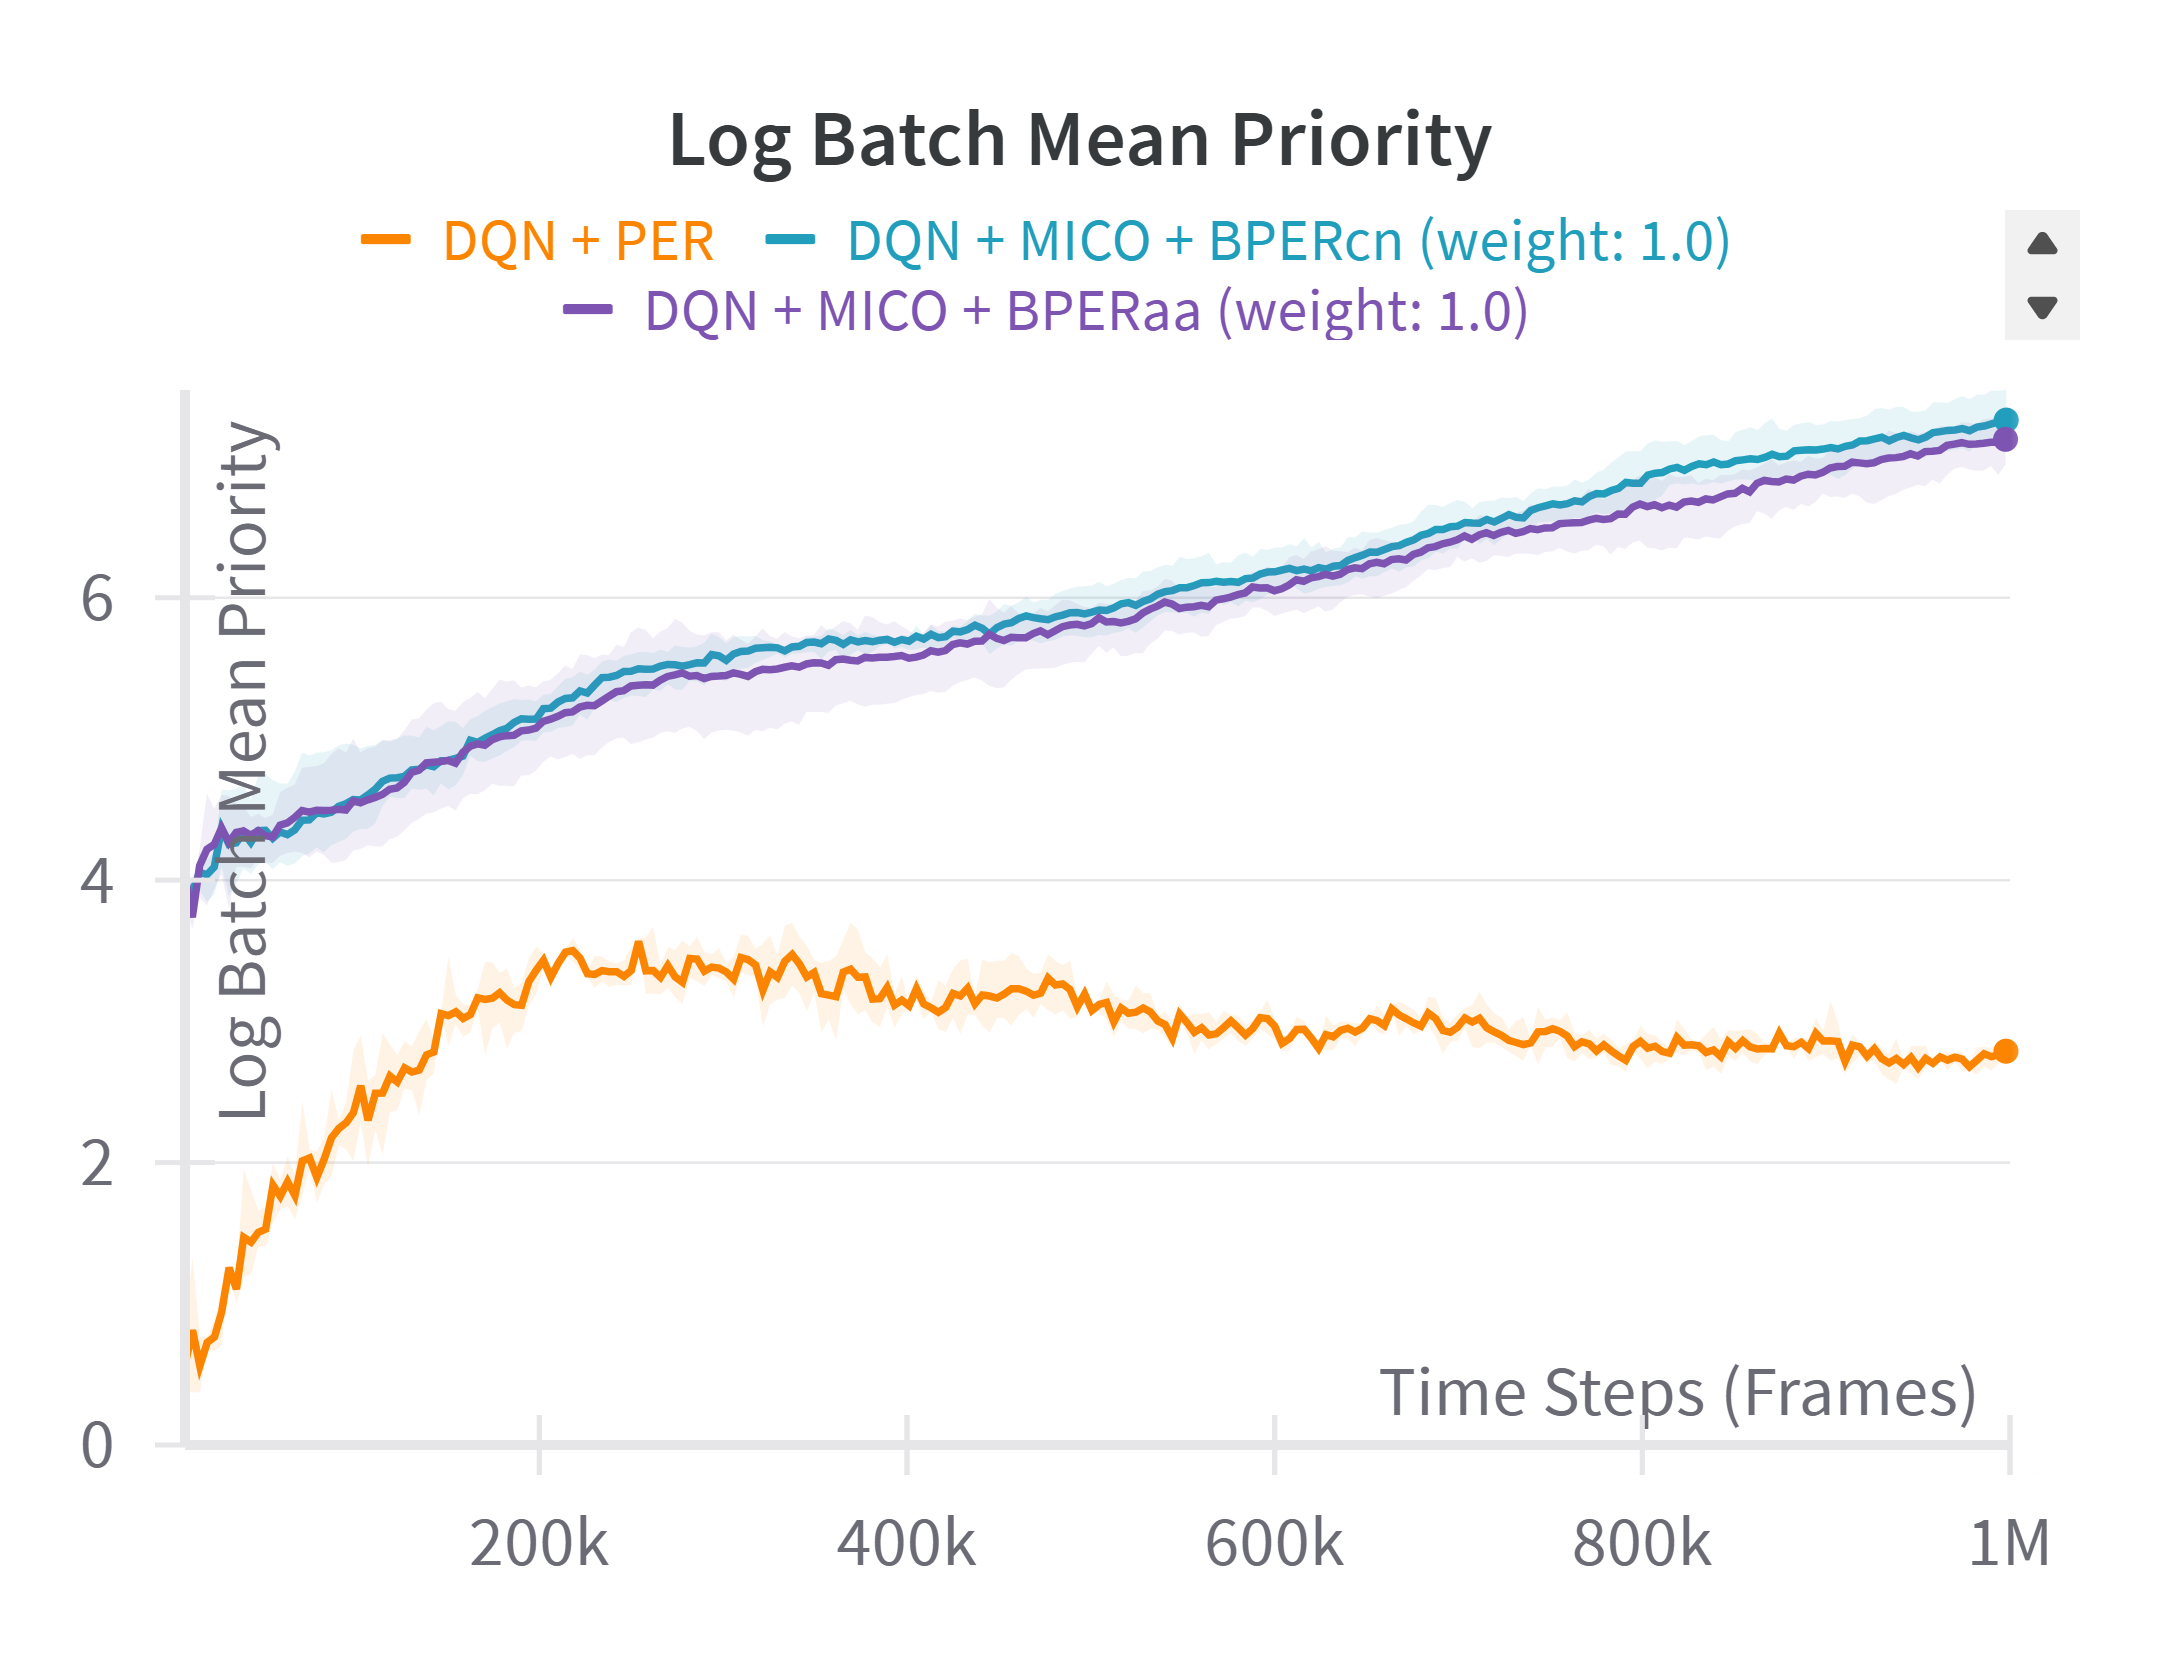
\includegraphics[width=\linewidth]{Results/general_results/log_mean_batch_priority_acrobot.png}
        \caption{Acrobot-v1}
        \label{fig:log_mean_batch_priority_acrobot}
    \end{subfigure}
    \caption{Two images side-by-side}
    \label{fig:log_mean_batch_priority_methods}
\end{figure}

\section{Summary Discussion}

The propose method yield promising results with some additional considerations to take into account. On the one hand, the GridWorld experiments help to empirically confirm our proof of concept by demonstrating the effectiveness and benefits of our proposed bisimulation strategies, BPERcn and BPERaa, in addressing three key problems: task-agnostic sampling, outdated priorities, and state space coverage.

\begin{itemize}
    \item The \textbf{task-agnostic sampling} section suggests that, although the TD-error serves as an indicator of potential improvement in the Q-values, it is insufficient as a proxy for expected learning progress in our GridWorld. In contrast, a notion of behavioral similarity proves to be a better indicator of expected learning progress.
    \item The \textbf{outdated priorities} section suggests that our proposal effectively alleviates the problem of outdated priorities by reducing the distance between the ideal and sampling probability distributions, even though the priorities are updated only in the current minibatch.
    \item The \textbf{state space coverage} section indicates that bisimulation strategies can encourage more exploration in the environment without explicitly instructing the policy to explore more, as is done with $\epsilon$-policies and other exploration mechanism \cite{amin2021survey,ladosz2022exploration}.    
\end{itemize}

On the other hand, the performance of our method in other domains is only slightly better and does not show consistently significant improvements. In some environments (e.g., CartPole), there are no clear performance gains over the DQN + PER. However, what remains consistent across experiments is that the bisimulation strategies outperform the direct baseline DQN + MICo, even if they do not surpass DQN or DQN + PER.

\begin{itemize}
    \item The cases where our method does not outperform DQN or DQN + PER (e.g., CartPole and Mountain Car with a priority weight of 1.0) appear to be related to \textbf{scenarios where DQN + MICo is not efficient}. When the MICo learning itself is ineffective, it is expected that our approach would also yield suboptimal results.
    \item The effectiveness of \textbf{our method is connected to the structure of the evaluated environments}, specifically the action space, transitions, and reward structure. In simpler environments such as CartPole and deterministic Mountain Car, the effective state space is smaller with few transition and the same rewards per time step, making it more challenging to identify behaviorally similar states for MICo learning.  In fact, results in simple Atari environments (e.g., Pong) from MICO reported by Castro et al. \cite{castro2021mico} do not show evident improvements.
    \item The \textbf{mean batch priority} is a viable indicator for analyzing the level of prioritization in each environment, showing that our proposal consistently encourage large priority values within the current mini batch. However, the results have different interpretations, which must be interpreted alongside the episode reward results to determine whether a high mean batch priority is having a positive impact or not.
\end{itemize}



